% $Id: report.tex 271 2003-05-02 16:04:07Z mackers $
\documentclass[a4paper,12pt]{report}

\title{SightWeaver - A Table Repair Tool
\\ \small \textcolor{red}{$Id: report.tex 271 2003-05-02 16:04:07Z mackers $}
} 
\author{David McNamara}
\date{2003}

\usepackage{color}
\usepackage[pdftex]{graphicx}
\DeclareGraphicsExtensions{.pdf,.mps,.png,.jpg}

\newcommand{\code}[1]{\ensuremath{#1}}
\newcommand{\todo}[1]{\textcolor{red}{TODO: #1}}
\newcommand{\url}[1]{\textcolor{blue}{#1}}
\newcommand{\strong}[1]{\textbf{#1}}
\newenvironment{abstract2}[1]{\addcontentsline{toc}{chapter}{Abstract}\vspace*{30mm}\begin{center}\subsubsection{Abstract}\end{center}}{}
\newenvironment{acknowledgements}[1]{\addcontentsline{toc}{chapter}{Acknowledgements}\vspace*{30mm}\begin{center}\subsubsection{Acknowledgements}\end{center}}{}

\begin{document}

\pagenumbering{roman}

\maketitle
\pagebreak

\vspace*{82mm}
\begin{center}
\strong{Sightweaver: A Table Repair Tool} \\
David McNamara \\
B.A.(Mod.) Information and Communications Technology \\
Final Year Project May 2003 \\
Supervisor: Alexis Donnelly 
\end{center}
\pagebreak

% $Id: abstract.tex 269 2003-04-22 14:45:04Z mackers $
\begin{abstract2}

Many tables of data on the web are designed purely for visual presentation
and do not contain semantic information about the structure and content of
that table. This presents problems for visually-disabled people who use the
Internet with adaptive technology such as screen readers.

This paper presents a design and implementation of a tool to analyse and repair
data tables in order for them to adhere to web accessibility standards. In
doing so, screen readers will be able to assist their users to understand
tables in an equivalent manner to non-visually disabled users.

This report looks at the motivation behind creating accessible websites and 
argues the benefits to disabled and non-disabled people alike. An overview
shows how visually disabled people use the web and various accessibility 
standards and legislation is studied.

A suitable design and implementation for a table repair tool is presented, as
well as the issues encountered while developing the tool. An analysis of the
system appraises the tool against accessibility standards and studies
the repaired tables using actual screen reader programs.

Finally, the conclusion evaluates the tool against the requirements and 
presents areas for further investigation.

\end{abstract2}

\pagebreak

% $Id: acknowledgements.tex 263 2003-04-16 17:34:13Z mackers $
\begin{acknowledgements}

The author wishes to thank the following people for their invaluable help
during the course of this project. Alexis Donnelly for the initial project idea
and patience and help during the successful completion and Santa Claus for
providing the author's first computer and inspiring him to pursue a career
in this area. Also thanks to Aidan Kehoe for providing the French version.

\end{acknowledgements}

\pagebreak

\tableofcontents
\pagebreak

\setlength{\parskip}{0.5em}

\pagenumbering{arabic}

\chapter{Introduction}
% $Id: introduction.tex 269 2003-04-22 14:45:04Z mackers $

\begin{quotation}

The true reason to design for accessibility is greed. Quite simply, I want it
all, and so should you. Give us everything you've got. Give us everything there
is to give.  \cite{joeclark}

\end{quotation}

It is estimated that in the United States alone 40.8 million individuals has
some sort of disability, and 27.3 million of those has a severe disability
\cite{webaim}. This represents some 10-20\% of the population, and this figure
is mirrored in most countries. As is shown in the next chapter, this represents
a significant portion of web traffic and should not be ignored.

The vast majority of websites currently on the web are designed solely with
sighted, non-disabled visitors in mind. Disabled visitors using assistive
technology\footnote{Assistive or adaptive technology can be defined as some
hardware or software that eliminates barriers to using a computer.} may or may
not have complete access to these sites. Because no non-visual information has
been provided, large sections containing images, multimedia or badly marked-up
HTML remain no-go areas.

The greatest shame is that, with a little extra work, website authors and
designers can greatly improve access to their site for all types of visitors.
The reasons that this isn't currently done can be attributed both to ignorance and
to apathy.

What \emph{can} be done, however, is to provide assistance to web publishers in
creating accessible web sites. One type of assistance is the promotion of
accessibility standards and guidelines in the form of documentation and books, 
of which plenty of available. Through these, web designers can 
educate themselves in the technical aspects of website accessibility and can develop
with this in mind with little extra effort. 

However, some aspects of website accessibility can be confusing and difficult
for the reluctant web designer, and impossible for the average content manager.
In an attempt to obviate some of this difficulty, a wide variety of tools
has been developed, ranging from simple accessibility checkers to elaborate
authoring environments and plug-ins. Some of these are discussed in the 
next chapter.

This report details the design and implementation of one such tool, which 
focuses on one particular aspect of accessibility; tables. 

\section{Objectives}

The primary objectives of this report are outlined below:

\begin{itemize}

\item To present the motivation behind the accessibility movement, both from a
social and legal perspective. A background of the demography of disabled web users
will be provided.

\item To explain the accessibility standards and legislation that exists today,
and the problem with existing websites.

\item To outline existing technologies, both assistive technologies and 
accessibility tools.

\item To propose a solution to one aspect of accessibility; tables. 

\item To successfully design and implement a tool which will assist authors
in creating fully accessible HTML tables.

\item To test the output of the tool with accessibility and legal standards.

\item To present a brief discussion on future developments in this area and 
how the tool could be improved.

\end{itemize}

\section{Structure of this Report}

There follows a brief outline of the structure of this report.

\begin{itemize}

\item This chapter has introduced the main concepts and the objectives of the report.

\item Chapter 2 will expand on the basic concepts introduced in the previous
chapter.  It will present some statistics on the numbers of disabled visitors
to websites, and present arguments as to why all websites should be fully
accessible, from a socially responsible and legal point of view. Important auxiliary
benefits will also be listed. 

The chapter will introduce the current state of web accessibility standards for
websites in general and tables in particular. It will also include a summary of
assistive technologies and tools and programs related to this report.

\item In chapter 3, the design for the table repair tool will be detailed. The 
user, domain and system requirements will be presented, and a suitable
architecture proposed.

\item The next chapter will show how the design was implemented throughout
the development cycle. A road-map will show how the implementation was planned
and any problems encountered will be identified together with their solutions.

\item Chapter 5 will be an analysis of the design and implementation of the
tool.  The chapter will show the results of thorough testing to accessibility
standards as well as an evaluation of the project's commitment to its
requirements.

\item 
The report will then conclude with a summary of what of achieved in the project
as well as a discussion of possible future work and developments.

\end{itemize}



\chapter{Background}
% $Id: background.tex 269 2003-04-22 14:45:04Z mackers $

\begin{quotation}
The power of the Web is in its universality. Access by everyone regardless of
disability is an essential aspect.
\end{quotation}
 -- Tim Berners-Lee, W3C Director and inventor of the World Wide Web

\section{Motivation}

Why Bother With Accessibility?

There are many reasons why most web developers don't concern themselves with
accessibility. Some of these reasons are perfectly valid, but most are
unfounded.

Most believe that visitors with disabilities represent such as small number of
total visitors as to render them insignificant. This perception is hard to
justify when one looks at the figures. As stated in the previous chapter, between 10\% and 20\%
of Americans have some type of disability. A Harris Poll released in
2000 showed that 43\% of these use the Internet, less than non-disabled people,
but considerable all the same. 

The Survey on Income and Program Participation (SIPP, 1999, carried out by the
U.S. Department of Commerce, Economics and Statistics Administration, National
Telecommunications and Information Administration) estimates that 56.7\% of
non-disabled people have Internet access. From these figures it can be derived
that between 2.4\% and 4.8\% of Internet users in the United States have some
degree of disability. 
%\todo{nice graph here?}

To put this in context, consider a popular website with a million unique
visitors a month. By not regarding accessibility, the website owners are
effectively denying full access to up to 48,000 people. 

In the context of this document, it is desirable to isolate people in this
category with some sort of visual impairment. The same Survey of Income and
Program Participation found that 3.5\% of Americans have vision problems, and 
21\% of these people have Internet access. That's about 1,542,410 people
who are not going to able to correctly see a website the way the designers
would. The numbers doesn't seem so abstract when a raw human figure is
put on it.

Another reason why accessibility is not implemented is the myth that it is
expensive. This only really holds true if it is done after the fact. Building
basic accessibility into the design in the first place is effectively free,
requiring developers only to add small amounts of extra code here and there, a
task which should be done without a second thought. In fact, in the long
term, it will probably save the company money in disability lawsuits and
other costs.

For instance, in Australia in June 1999, Bruce Maguire lodged a complaint with
the Human Rights \& Equal Opportunity Commission (HREOC) under a law called the
Disability Discrimination Act. His complaint concerned the Website of the
Sydney Organising Committee for the Olympic Games (SOCOG), which Maguire
alleged was inaccessible to him as a blind person. Maguire successfully won the
case, and the SOCOG was fined \$20,000 in Australian dollars. It was argued
that building accessibility into the project afterwards would have cost A\$2.8,
but experts believe that incorporating it from the start would have only added
2\% to the cost.

Companies must already provide for minority groups. Religious holidays and customs
must be honoured and company buildings must be properly accessible, so
why not websites?

Additionally, a conscious effort is made by website developers to make their
website `accessible' to users of different browsers. So, in that respect, they
must recognise the diversity on which the web is founded, and so should have no
problem envisioning alternative versions of their website. The problem may in
fact be a very basic human fear; ``To imagine your site as experienced by a
blind person is to imagine you are blind yourself.''\cite{joeclark}

The bottom line, however, is that a level of social responsibility must be
applied by website designers and content developers. Although technically
impossible, if a website were to discriminate between different races or
against women, then there would be uproar, so why should discrimination against
people with disabilities be different? 

\section{Legal Requirements}

In most developed countries today there is anti-discrimination legislation
which forbids discrimination or unequal treatment on the basis of disability.
While in most cases this legislation predates the popular uptake of the web, in
general it can be applied to the web (see Olympics example above). Furthermore,
in certain jurisdictions, there is now an explicit requirements for government
departments' and agencies' websites to be accessible. Two such examples are
touched on below.

\subsection{Section 508}

\begin{quotation}

Section 508 requires that Federal agencies' electronic and information
technology is accessible to people with disabilities. The Centre for
Information Technology Accommodation (CITA), in the U.S. General Services
Administration's Office of Government-wide Policy, has been charged with the
task of educating Federal employees and building the infrastructure necessary
to support Section 508 implementation.\cite{section508}

\end{quotation}

The guidelines themselves are similar to W3C's Web Content Accessibility
Guidelines but obviously with a more legal slant. Within the last year Section
508 has come into law, requiring all government websites (with a few minor
exceptions) to comply. 

Additionally, any private sector companies that want to sell to the United
States Government would presumably adhere to these standards. After that,
other private companies might start to take notice.

\subsection{Irish Government Web Publication Guidelines}

In 1999, the Department of the Taoiseach launched Web Publication Guidelines
for Public Sector bodies\cite{irishgov}, with the target for all Government
Department web sites to achieve level AA compliance (see section on Web Content
Accessibility Guidelines) by the end of 2001. A 2002 Web Accessibility in
Ireland Study\cite{warp2002} showed that 100\% of public service websites
failed to meet the WCAG AA accessibility level, proving that a lot of work is
needed.

The guidelines themselves have been compiled by the National Disability
Authority\cite{nda:accessit}, and are generally aligned with W3C's WCAG
guidelines.

\section{Auxiliary Benefits}

Apart from the social and legal liabilities that accessibility negates, they are
a number of auxiliary benefits which may not be entirely obvious, both for the
website owner and for disabled and non-disabled visitors.

Apart from the actual increase in overall visitor numbers by enabling access to
people with disabilities, you may also attract visitors that may not actually
have come in the first place. For instance, blind shoppers may prefer the
comfort and ease of shopping online rather than face the difficulty of getting
in town and navigating real-world shops. Similarly, accessible websites for
hotels allow disabled users to research travel plans and any special
requirements they may need. In effect, these websites can make business gains,
that otherwise wouldn't have existed.

In practice, making a website accessible can have all sorts of other benefits. 
Usually, this very act ensures that the website is of a better quality than its
inaccessible rivals. In general, accessible websites afford a greater level
of standards compliance and logical emphasis, a trait which is picked up by
search engines which look for structural headings to rank a site and index
textual equivalents of images and multimedia, thus boosting targeted traffic
to your website.

The use of image descriptions and the separation of content and presentation
via CSS\footnote{Cascading Style Sheets allow the website's style to be placed
in a separate file which only needs to be downloaded once for the whole site.}
leads to a reduced download time, which is beneficial both to the server's
bandwidth use and to visitors with slow connections. It also means that, should
they wish, users may safely turn images off or easily view the website in
alternative browsers, such as mobile phones and kiosks.

\section{How People with Visual Impairments Use the Web}

Visually disabled users range from from the colour blind to the fully blind.
Table accessibility does not adversely affect the colour blind, who are still
able to see the table structure. Similarly, people with a relatively modest
visual impairments may use a screen magnifier to blow up the size of text,
images, tables and everything else on the screen. They are essentially seeing
the same table structure as a non-visually impaired person, and do not need to
make use of any extra information about the table structure.

Visitors that are totally blind, i.e. don't actually use the computer monitor
use something called a \emph{screen reader}, which is a program that reads or
speaks aloud a description of the website consisting of, but not limited to,
the textual content, descriptions of images and multimedia, `meta' information,
links, and table structural information. While most screen readers are robust
enough to handle even the most badly-formed website, they rely on good
authoring to give the user extra clues as to the exact make-up, structure and
meaning of the website.

A small majority of visually impaired users use braille display - a tablet
consisting of nylon or metal pins controlled by software to give tactual
feedback to the user. Braille software also uses the accessible content and
structure to convey the website to the user.

\section{Accessible Web Design}

\begin{quotation}

The World Wide Web Consortium's (W3C) commitment to lead the Web to its full
potential includes promoting a high degree of usability for people with
disabilities.

WAI, in coordination with organisations around the world, pursues accessibility
of the Web through five primary areas of work: technology, guidelines, tools,
education and outreach, and research and development. \cite{w3c:wcag}

\end{quotation}

Since 1999, the W3C has been working on its Web Accessibility Initiative (WAI).
One of the primary purposes of the WAI is to set out guidelines for
accessibility in web content, authoring tools and in user agents. For the
purposes of this document, the recommendations on web content and authoring
authoring tools are interesting. 

The WAI's Web Content Accessibility Guidelines ``explain how to make Web content
accessible to people with disabilities. The guidelines are intended for all Web
content developers (page authors and site designers) and for developers of
authoring tools.''\cite{w3c:wcag} 

From a technical point of view, these guidelines appear very abstract and so
two more recommendations are provided. The first is \emph{Techniques for Web
Content Accessibility}\cite{w3c:wcagtechs}, which reiterates the above document
from a technical perspective while providing points to the relevant sections in
the more detailed guidelines on individual web technologies. The second set of
recommendations, \emph{HTML Techniques for Web Content Accessibility
Guidelines}\cite{w3c:wcaghtmltechs} is a detailed technical document on how to
implement the above accessibility guidelines in the actual HTML or web content. 

By closely following the guidelines in these documents, web authors can develop
websites that are accessible to people with all sorts of disabilities.
Developers of web site authoring tools, including accessibility validators and
repair tools should use the guidelines to ensure that their programs only
output accessible web content.

\subsection{Web Content Accessibility Guidelines}

The Web Content Accessibility Guidelines cover most elements of a typical
website. Below are described some of the salient points, with the exception
of tables, which are described in more detail in the next section.

Each checkpoint has one of three \emph{priority} levels attached.  Level one
priority checkpoints are basic requirements for accessible websites and
\emph{must} be implemented by content developers. Addressing level two
checkpoints will remove significant barriers to accessing web documents, and
\emph{should} be implemented by content developers. Priority three checkpoints
\emph{may} be satisfied by websites as they will further improve web
accessibility. Websites conforming to these standards can be said to have a
\emph{conformance level} of A, AA or AAA respectively.

The following checkpoints have not been labelled with their
recommended priorities, as the table repair tool will strive to create level
three priority HTML. 

The first guideline is to provide equivalent alternatives to auditory and
visual content. This means that all images, pre-recorded audio and video should
have a text equivalent to allow access both to visually impaired visitors and
to those with reading or cognitive disabilities. For instance, in HTML, every
image should contain an ``alt'' attribute containing a textual description of
the image. Guideline 6 is related to this and requires that new technologies
such as CSS, scripts, applets and frames do not render the page inaccessible,
and that there should be alternative content, if appropriate. Furthermore,
Guideline 8 states that any embedded content that has its own interface
should also be fully accessible.

The second guideline states that colour shouldn't be relied upon to convey
information. For example, links should not be styled using colour alone, 
as users with colour-blindness may not be able to distinguish linked text from
non-linked text.

Guideline 3 requires that markup and style sheets are used correctly. This
guideline encompasses a range of checkpoints including ensuring that the HTML
is well-formed and validates to a standard grammar\footnote{HTML grammars are
sets of standards, e.g. HTML 4.01 to which websites state their adherence by
specifying a document type declaration.}, and that headers, lists, quotations
and tables are marked up in HTML using their intended tags. This ensures
alternative browsing devices can intelligibly understand the organisation of a
page. This guideline also encourages use of CSS style-sheets to store the
style and presentation of a website, freeing other agents from having to
decipher in-line presentation tags.

Natural language use should be identified by declaring the primary language for
the document in general, as well as any other languages used. This allows
speech synthesisers to choose how the text is pronounced. It also allows search
engines to find key words in the particular language used. In practise, content
developers should use a ``lang'' attribute on the HTML element and any other
elements as necessary. Additionally, abbreviations and acronyms should have
their full meaning described using a ``abbr'' or ``acronym'' tag.

Guideline 5 is concerned with ensuring tables transform gracefully and is 
covered in detail in the next section.

The remainder of the guidelines are more abstract, stating that websites are
designed without any specific device in mind (e.g. mice), remain compatible
with known assistive technology shortfalls, and provide context, orientation
and navigation information. 

Naturally, it is also recommended that websites adhere to the other W3C
guidelines and technologies.

\subsection{Accessible Tables}

Guideline 5 is especially interesting in the context of this report as it
encourages the correct markup of tables so that they can be correctly
``transformed'' by accessible browsers and other assistive technologies.

``Tables should be used to mark up truly tabular information (``data
tables'')''\cite{w3c:wcag}, meaning that tables used to layout web
pages should be avoided, as these may cause problems for users of
screen readers.

The following checkpoints are also recommended:

%\todo{sample HTML table containing all these checkpoints and reference in each section to the table}

\subsubsection{Provide Summary Information}

All tables should have summaries. In HTML, these can take the form of a
``caption'' element to describe table in two or three sentences, e.g. ``Number
of civilians killed in the war''. A caption may not always be necessary.

A summary of the table should be provided via the ``summary'' attribute. The
purpose of the this is to describe the relationship among cells, including
their headers, spanning information or ``other relationships that may not be
obvious from analysing the structure of the table but that may be apparent in a
visual rendering of the table''\cite{w3c:wcag}. The summary may also be used to
describe the context of the table in terms of the entire document. An example:
``This table charts the number of civilians killed per day in the war and to
which side they belonged. The first row lists the three nationalities involved
in the war and the first column lists the dates in which they were killed
ranging from 17th March to 21st April''.

\subsubsection{Specify Table Headers}

The table's logical headers must be marked up as headers, i.e. in HTML, data
cells should use ``td'' tags and header cells should use ``th'' cells. 

Repeated rows of headers should be placed in a ``thead'' element and repeated
rows of footers (merely headers at the bottom of the table) should be placed
in a ``tfoot'' element.

\subsubsection{Specify Header Cell Associations}

Table elements should be labelled with appropriate markup to identify the
relationship between data and header cells. Each data cells should have one or
more related headers to which the data in that cell pertains. A ``scope''
attribute can be applied to a table header to imply that this header is
authoritative for cells below it (``col'' scope) or to the left of it (``row''
scope). For more complex tables, data cells can also be labelled with the
``headers'' attribute in order to indicate a relationship with one or more
individual headers.

A third attribute, ``axis'' may be used to label cells so that future browsers
and agents will be able to select data from a table by filtering on 
categories.

\subsubsection{Provide Header Label Abbreviations}

For headers with long descriptions, an ``abbr'' attribute should be used to
give a terse abbreviation so that future screen reading browsers which can read
row and column headers for each cell can cut down on reading time and
repetition.

\subsection{Authoring Tool Guidelines}

The W3C also provides guidelines for developers creating \emph{authoring
tools}\cite{w3c:atag}. An authoring tool can be defined as a program used
to create web content, including:

\begin{itemize}

\item ``WYSIWYG''\footnote{What You See Is What You Get} HTML, XML and CSS
editors.

\item Tools that have the option as saving in a web format (i.e. word 
processors or desktop publishing content)\footnote{It should be noted at
this stage that the most popular word processor, Word, is in breach of 
almost every Authoring Tool Guideline.} and third party tools that
convert these formats to web formats.

\item Tools that produce multimedia where it is intended for use on
the web.

\item Tools for site management for site publication, including tools
that automatically generate web content from databases, and tools
that convert from one format to the other.

\end{itemize}

Since most web content is created using an authoring tool of some description,
they play a critical role in ensuring the accessibility of the web. To this
end, ``authoring tool developers must take steps such as ensuring conformance
to accessibility standards (e.g., HTML 4), checking and correcting accessibility
problems, prompting, and providing appropriate documentation and help.''

A summary of W3C's authoring tool guidelines follows:

\begin{enumerate}

\item Authoring tools should support accessible authoring practices. That is,
authoring tools should generate accessible content and not introduce any
non-accessible content. If the tool imports, transforms or converts existing
content, it should preserve any existing accessibility information.

\item Authoring tools should generate well-formed, valid markup using 
existing W3C standards.

\item The creation of accessible content should be supported. I.e. the author
should be allowed to input text equivalents, captions, auditory descriptions,
etc. that ensure that the final version is accessible. Where mandatory
information is needed, the author should be prompted.

\item Ways of checking and correcting inaccessible content should be provided.
The user should be informed of inaccessible content and assisted in correcting
these problems. Any markup not recognised by the tool should be preserved.

\item The tool's accessibility features should be part of the program's overall
``look and feel'' so that the author easily accepts these features as part
of the operation of the program.

\item Accessibility should be promoted in the help and documentation.

\item The tool itself must be accessible to authors with disabilities using
existing operating system accessibility standards and conventions. 
%\todo{see appendix b?}

\end{enumerate}

\section{Related Work}

\label{relatedwork}

Below is a short list of validators and tools to be used by web content
developers to make their websites more accessible. The list is limited to the
most feature-rich and effective validators and tools that specialise in
table accessibility.

For each tool a brief description is given as well as its features and
limitations, if any. By showing the current state-of-the-art and the limits
there of, this section hopes to justify this report's objective of creating a
tool which will overcome some of these difficulties.

\subsubsection{Bobby}

Bobby is a web accessibility validator ``designed to help expose and repair
barriers to accessibility and encourage compliance with existing accessibility
guidelines.'' It comes in a desktop or an online form and can check single
web-pages or whole sites against WCAG or Section 508 accessibility guidelines.

More information: http://bobby.watchfire.com/

\subsubsection{The Wave}

The WAVE is a free online tool that ``facilitates human judgement in the
accessible design process.'' For a given website, it will `flag' all elements
in the web page and indicate possible problems using different icons.

More information: http://www.wave.webaim.org/

\subsubsection{W3C HTML Validation Service}

While not strictly an accessibility validator, W3C's HTML Validation Service
checks HTML and XHTML web pages for conformance to W3C standards. It is
useful for ensuring that web pages are well-formed and do not contain
any invalid markup.

More information: http://validator.w3.org/

\subsubsection{Tablin}

Tablin is a program that can linearise HTML tables. It displays a textual
version of a table similar to what a screen reader may produce. 

The tool is useful for testing tables to make sure they make sense when
linearised, but does not seem to take in account the full suite of accessible
features, such as headers associations, and so may not be entirely useful for
the purposes of this document.

More information: http://www.w3.org/WAI/References/Tablin/

\subsubsection{Accessify.com's Accessible Table Builder}

This tool lets users create fully accessible tables from scratch. The user
may specify the cell's structure including height, width, headers etc. as well
as the table summary, caption and the data itself and the tool will return
fully accessible table HTML.

The main problem with this tool is that is does not allow the import of
existing tables/documents, requiring tedious cell-by-cell input. It also does
not permit complex header hierarchies, cell axes or header abbreviations.

More information:\newline
http://www.accessify.com/tools-and-wizards/accessible-table-builder\_step1.asp

\subsubsection{A-Prompt}

A-Prompt (or Accessibility-Prompt) is a free software tool designed ``to improve
the usability of HTML documents by evaluating Web pages for accessibility
barriers and then providing developers with a fast and easy way to make the
necessary repairs.''

The program itself is quite sophisticated, allowing the user to check web pages
against all W3C and Section 508 conformance levels. The author has full control
over accessibility features such as text equivalents, form accessibility and
table accessibility.

Its table support is reasonable, allowing the user to enter summary and caption
information for each table and abbreviations for each header. However it only
recognises headers in the first row or first column, so more complex tables
are not supported. Also, while it recognises the absence of header scopes
and associations, it does not allow in-line editing and suggests that the
author add these manually.

More information: http://aprompt.snow.utoronto.ca/

%\subsubsection{WebAIM.org's Screen Reader Simulation}

%More information: http://www.webaim.org/simulations/screenreader



\chapter{Design}
% $Id: design.tex 269 2003-04-22 14:45:04Z mackers $
\section{Requirements}

This chapter will outline the requirements of the table repair tool from
a user, domain and system point-of-view.

\subsection{User Requirements}

\label{userreqs}

\subsubsection{Importing Documents}

\strong{The user will be able to import documents using a standard open dialog
box.} The application supports any document authored in Word 97, Word 2000,
Word XP, Excel 2000, Excel XP, FrontPage or Dreamweaver. Documents saved in
future versions of these applications as well as any reasonably well-formed
generic HTML should also be anticipated and supported. The application may be
later extended using external import filters to support other formats such as
CSV or RDF. The CSV filter will be implemented as an example of how to do this.

Upon selecting the document to import, the application will display the
table(s) in that document, ready for editing or exporting. Only one document
may be opened simultaneously.

\subsubsection{Document Content}

\strong{Document content outside of tables will not appear in the application
window, but will be preserved in the output document. Furthermore, this content
will be converted to valid XHTML 1.0 Strict.} This may mean some structure may
be altered to become more structured and/or accessible, however no content will
be lost in the conversion. Exported XHTML documents will be \emph{cleaned} to
remove font tags and change presentational tags to logical tags. Other (non
XHTML) output formats may discard non-table content.

\strong{Styles and formatting in the table itself will not appear in the
application window.} This is to reduce visual congestion and to emphasise the
table headers when displaying the table (these are displayed in bold). The
structure (i.e. HTML markup) of individual cells may change in the conversion
process in order to conform to the XHTML 1.0 Strict standard or to maintain the
same level of accessibility across the table. For example, bold tags will be
changed to strong tags. However, fully accessible HTML for non-table elements
is outside the scope of this application. If possible, the user should avoid
including non-table elements (e.g. images, fonts and embedded objects) in the
input documents.

\subsubsection{Table Structure Preservation}

\strong{The existing table structure and attributes will be preserved during
the importation process.} The imported table(s) will have the same number of
rows and columns as the original document. The table's summary, caption and
other attributes will be preserved.

\subsubsection{Table Header Identification}

\strong{The document parser will make a reasonable attempt to identify the
headers and sub-headers for each table and display the headers for the user to
verify or adjust.} This will be achieved using any existing header markup in
the original document. If no existing markup exists, the parser will attempt to
identify headers by examining other markup and styles. No distinction is made
between headers and sub-headers.

\subsubsection{Table Navigation}

\strong{The application supports multiple tables in the document, and will
provide a mechanism for switching between tables.} A maximum of ten tables is
supported. Nested tables (i.e. a table inside another table) and tables for
layout purposes are not supported. Documents containing either of these types
of table will not be imported.

\subsubsection{Specifying Table Information}

\strong{For each table in the document, the user shall be able to specify the
table summary and caption.} This functionality will be provided using text
input boxes in separate dialogs. The application will \emph{not} provide
default values for these required data fields in order to encourage the user to
enter these values. The application will not export a document containing
tables that have no summary or caption information.

\subsubsection{Cell Highlighting}

\strong{Multiple cells may be selected in order to perform an operation on more
than one cell}. By using the shift key or other modifier, it will be possible
to highlight or select multiple cells. Certain operations can then be performed
on this group of cells.

\subsubsection{Header Associations}

\strong{It will be possible to manually edit the header associations for each
cell or group of cells using a separate dialog box.} This will allow expert
control over each cell, by giving the user access to the internal hierarchal
structure of each table. This is achieved by referencing associated header(s),
using their unique identifiers. This text box is accessed via a menu item and
is available for both normal cells and for headers cells (which may in turn
have super-headers). Cells may have associations with one header or with many
headers or sub-headers on preceding rows or columns. 

\subsubsection{Header Information}

\strong{It will be possible to edit the abbreviation, ID and axis for any
header.} This information can be edited via separate dialog boxes accessed
from a menu. Abbreviations will be limited to 10 characters and may not exceed
the length of the header label. Header IDs are automatically assigned. Cell
axes are optional.

\subsubsection{Status Bar}

\strong{Information on the currently highlighted cell(s) is displayed in a
status bar.} For normal cells, the header associations and the cell axis (if
any) is displayed. For headers, the ID and the header abbreviation will also be
displayed.

\subsubsection{View Source}

\strong{The current document source will be available via a menu item}. The
source will be displayed in a separate window and will reflect the state of the
document's tables at that moment in time. The source will be in XHTML
regardless of what export format the user ultimately chooses.

\subsubsection{Exporting Documents}

\strong{When the user judges the structure of the table(s) is satisfactory, the
user shall export the document using a standard `Save As' dialog}. The default
output format is XHTML 1.0 Strict. 

Other output formats may be implemented at a later stage and will be included
in this dialog. Examples of other output formats are CALS\footnote{CALS is the
table structure used by the DOCBOOK format} and HTML 4.0.

The application will be able to re-import exported documents, however it is not
required that the application retain the header association information that
has been saved, and so these documents will be treated like generic XHTML.

%\subsubsection{Command Line Scripting}

%\strong{It will be possible to autonomously and automatically instruct the
%program to perform conversions from the command line.} This will be only
%possible with documents containing one table and requires that some
%information be passed to the program as command line arguments, such as the
%table summary and caption. The quality of this result will vary depending on
%the input document and the program's ability to identify headers in the
%document. So, while results may not be as accurate as the interactive method,
%the program may be interfaced with other applications or on websites.

\subsection{Domain Requirements}

\subsubsection{XHTML 1.0 Strict Compliance}

The primary output format is HTML. The HTML is intended to be as accessible as
possible. Rather than choosing a pure HTML standard, such as HTML 3.2 or HTML
4.0, the program will use the XHTML~\cite{w3c:xhtml} output format. 

\begin{quotation}

The Extensible Hypertext Markup Language (XHTML) is a family of current and
future document types and modules that reproduce, subset, and extend HTML,
reformulated in XML. XHTML Family document types are all XML-based, and
ultimately are designed to work in conjunction with XML-based user agents.
XHTML is the successor of HTML, and a series of specifications has been
developed for XHTML.

\end{quotation}

XHTML has a number of benefits over standard HTML:

\begin{itemize}

\item XHTML documents are XML conforming. This means that they can be edited,
viewed and validated with existing XML applications.

\item XHTML documents can seamlessly be viewed and parsed by existing HTML
tools and browsers.

\item XHTML documents can be parsed using the document object model, allowing
for automated scripts or agents better access to the content of the document.

\item XHTML is rapidly being accepted as the replacement for HTML, with new
standards and tools being development to take advantage of the format.

\end{itemize}

As XHTML can be parsed by existing and older browsers, the end user should not
be concerned that the document is actually XHTML. Instead it makes sense to use
this newer standard in order to avoid future deprecation. What's more, because
the DOM is extensively used to manipulate the source documents, XHTML is
explicity implied, which simplifies the generation of the output document.

\subsubsection{W3C Web Content Accessibility Guidelines 1.0}

The W3C Web Content Accessibility Guidelines~\cite{w3c:wcag} (also known as the
Web Accessibility Initiative (WAI) Guidelines) explain how to make web content
accessible to people with disabilities. They are intended to advise page
authors, site designers and developers of authoring tools on how to make web
content more available to all users, whatever user agent they are using or
constraints they may be under. 

The output document will conform to Guideline 5, which is ``Create tables that
transform gracefully''. It is advised to ``ensure that tables have necessary
markup to be transformed by accessible browsers and other user agents.''

As a secondary objective, a reasonable attempt will be made to ensure
that the rest of the document conforms to some of the other guidelines in this
document, specifically those that can be automated, as no data will be obtained from
the user on these elements.

This document will also extensively make use of W3C's document on Techniques
for Web Content Accessibility Guidelines~\cite{w3c:wcagtechs}, which includes
methods and techniques for satisfying the requirements defined in ``Web Content
Accessibility Guidelines 1.0''.

\subsubsection{Section 508 Compliance}

In 1998, the United States Congress amended the Rehabilitation Act to require
their electronic and information technology accessible to people with
disabilities. Section 508~\cite{section508} is the manifestation of this
amendment.

The output document will conform to part 1194.22 of this document governing
``Web-based intranet and Internet information and applications''.

\subsubsection{Irish Government Website Accessibility Regulations Compliance}

The Irish Government's Public Service Web Standards states that Irish public
service web sites must conform to the WAI Guidelines and the Irish Public
Service Meta-data Standards~\cite{irishgov}.

While it has been established that the document will conform to WAI Guidelines, it
will also be ensured that the meta-data standards are maintained.

\subsubsection{W3C Authoring Tool Accessibility Guidelines} 

The W3C also provides guidelines for developers creating \emph{authoring
tools}\cite{w3c:atag}. The program will adhere to these guidelines.

By its very nature the program will support accessible authoring practices
which will be part of its look and feel. The produced output will be valid
XHTML and have no non-accessible content. The program will not output a file
that contains non-accessible tables, and will prompt the user in this case.
Additionally, each dialog box will document whatever feature it pertains to.

The program itself must also be accessible to people with disabilities. To do
this, it will make full use of the Java Accessibility Utilities, which are a
set of utility classes that help assistive technologies provide access to GUI
toolkits that implement the Java Accessibility API.

%\todo{More details on Java Accessibility API.}

\subsection{System Requirements}

\label{sysreqs}

\subsubsection{Window Appearance}

The main application window is not unusual in that it consists of a title bar, a
menu bar, a status bar and a content pane. When the application is first
loaded, the content pane and status bar will be blank, and the title bar will
have an enabled `File' menu and a  disabled `Table' and `Cell' menu. The `File'
menu will have enabled `Import' and `Exit' menu items and disabled `Export' and
`View Source' menu items.

Importing a document will cause the `Export' and `View Source' menu items and
`Table' and `Cell' menus to become enabled. The state of the menu items of the
latter two menus depends on what cells are selected. It is not possible to
close a document once it has been opened, but another document may be imported.

The look and feel of the application will use Swing's system dependant look and
feel. For example, when running the application on Microsoft Windows, the
application will use Windows' native widgets, icons and cursors.

Each user interface string will be read from a separate Java properties file.
This will allow easy localisation of the application into other languages.
A French version of the program will be provided as an example of how to
localise.

\subsubsection{Importing Documents}

The import feature is accessed via an `Import' menu item in the `File' menu.
Selecting this item will open up a standard `File Open' dialog box from which
the user may select a document. The default filter is `HTML Files' which
includes all files with `htm' in their extension, e.g. .htm, .html, .xhtml,
.HTML. Other filters included are `CSV files (*.csv)', `RDF files (*.rdf)' and
`All Files'. 

If a document is already open that has not yet been exported then a
dialog will ask the user if the open document should be exported first.

Each supported document type has its own \emph{Importer}, which knows how to
handle that document format. Each importer is an implementation of a common
interface, and so share the same methods and return types. The importers are
given the inputstream connected to the document that is being imported and are
expected to return a document object, which can then be handled uniformly by
the remainder of the import process.

The type of importer to use is determined by the document's extension. The file
extension is the part of the filename after the last period. For example, in
`index.html', the extension is `html'. Each supported importer and its
associated extension and import techniques is described below. Files with no
extension or an unrecognised extension are assumed to be HTML and thus use the
HTML Importer. File extensions are listed and match in both upper- and
lower-case forms, or a combination of the two.

The import process may take a short while to complete. In order to inform the
user that something is happening, the mouse cursor changes to its `wait' state
for the duration.

\subsubsection{The CSV Importer}

The CSV (Comma Separated Values) file format is a plain text file consisting of
multiple lines of data. Each line consists of a number of fields of data
separated by commas. Each field may be enclosed by double quotation marks. CSV
lacks any mechanism for distinguishing between header and content data, so is is
assumed that all the data is content. The CSV format is a supported output
format of a number of applications, such as Microsoft Excel and various
database systems, and so it would be desirable to support this import format.

The CSV Importer is implemented as a subclass of the XHTML Importer (see
below). This may seem strange, but in practise it is useful to use the XHTML
Importer's routines after the CSV has been converted to XHTML. This is done using
Doug Tidwell's CSV to HTML
converter\footnote{http://www-106.ibm.com/developerworks/xml/library/x-xmlexperts-csv/}.

The CSV Importer is used for any document with the `.csv' extension.

\subsubsection{The RDF Importer}

RDF (The Rich Text Format) is a standard document format used for distributing
documents among workgroups where Microsoft Word or any other proprietary
document format is not universally supported. RDF can be outputted from
Microsoft Word and other popular word processing software.

The RDF Importer will not be implemented at this stage, but hooks in the code
will allow the class file to be implemented and inserted at some later time. If
the filter is not found, then an exception will be thrown and an appropriate
error message will be displayed.

\subsubsection{DOC and XLS Documents}

The program will not support Microsoft Word's or Microsoft Excel's native
proprietary format (with `.doc' and `.xsl' extensions respectively). Any
attempted by the user to load one of these document will result in the display
of an error message inform the user that the program cannot read these file
formats and to use Word's or Excel's \emph{Save As HTML} feature.

\subsubsection{The XHTML Importer}

Documents with an `.xhtml' extension are opened using the XHTML Importer.
Because XHTML is a XML format, Java's XML parser can be used to open the
document, which will construct a document object from the file. If the XHTML
file is not well-formed, then an exception will be thrown and an error message
will be shown. XHTML documents with a different extension will be handled by
the HTML importer (see below), which will ultimately return a copy of the
original document.

\subsubsection{The HTML Importer}

Other files with an extension containing the string `htm' (e.g. `.htm',
`.html', `.shtml' and `.HTML') as well as files with unknown or missing
extensions are opened with the HTML Importer. The HTML Importer parser then
uses the following steps to create the document object.

\begin{enumerate}

\item Because this filter is the default filter, it must be verified that the file
is in fact HTML. To do this, the file is searched for an opening tag.  Any
particular opening tag cannot be searched for ( for example, `head' or `body')
as the HTML file may only be a fragment of another complete HTML file. This may
occur, for example, if the user copies out a table and pastes into a new file. 

Instead any opening tag is searched for, in the form of a less than sign ($<$)
followed by one or more alphanumeric characters and a space or greater than
sign ($>$). If one of these is found, it is assumed that the file is HTML. Of
course, this may occur coincidently in another non-HTML file. 

If the file does not appear to be HTML, and exception will be thrown and an
error message is displayed.

\item Next, the type of HTML document is determined. This is in order to run the
document through the correct \emph{preparser} (see below). It may be accurately
determined in which program the document was authored in (if any) by looking at
the `generator' meta tag. For example, documents authored and saved as HTML in
Word 97 have the meta tag\\ \code{<META\ NAME=``Generator''\ CONTENT=``Microsoft\
Word\ 97''>}\\. Now that is has been determined that this document was created in
Word 97, the preparser can be given clues on how to treat this file.

The exact format of the generator tag may vary slightly, e.g. use of double or
single or no quotes in either the name or content or both attributes, or and
upper- or lower-case `generator' attribute. A \emph{regular
expression}\footnote{Regular expressions are a standard way to search for
patterns in text strings, and are implemented in Java version 1.4 and later.}
will be used on the whole document string to pull out the generator tag.

Although unlikely, if may be possible that the document was saved in a version
of Word, and edited later by hand. This would leave the generator tag, but the
HTML source may not match what was expected from the Word version. In this
case, the robustness of the HTML parser will handle this to a certain extent
without a preparser.

\begin{table}
\begin{center}
\begin{tabular}{ll}
\strong{Product Version} & \strong{Generator Tag} \\
Microsoft Word 97 & Microsoft Word 97  \\ 
Microsoft Word 2000 & Microsoft Word 9 \\ 
Microsoft Word XP & Microsoft Word 10 \\ 
Macintosh Word 98 & Microsoft Word 97/98 \\
%Macintosh Word 2000 & \todo{word2kmac Generator Tag} \\ 
%Macintosh Word XP & \todo{wordxpmac Generator Tag} \\ 
Microsoft Excel 97 & Microsoft Excel 97 \\
Microsoft Excel 2000 & Microsoft Excel 9 \\
Microsoft Excel XP & Microsoft Excel 10 \\
%Microsoft Frontpage & \todo{frontpage tag} \\
%DreamWeaver & \todo{Dreamweaver tag} \\
\end{tabular}
\end{center}
\caption{Generator tags written by different programs}
\label{table:generators}
\end{table}

The type and version of HTML may also be determined using the document's
\emph{DOCTYPE}, if present. The DOCTYPE is a special tag that may or may not
occur in HTML files and will always occur in XHTML files. Using the DOCTYPE it 
can be determined if the file is HTML or XHTML and what version of that format. An
example of a DOCTYPE is $<$!DOCTYPE\ HTML\ PUBLIC\ ``-//W3C//DTD\ HTML\
4.0\ Transitional//EN''$>$. From this it is known that the document is HTML 
version 4.0 Transitional. As all the supported programs correctly output a
generator meta tag, DOCTYPE checking does not need to be implemented.

\item If the previous step identified a supported generator, then the document
can be run through a relevant preparser. Each supported program will have a
corresponding preparser. 

The purpose of pre-parsing is to ensure that successive stages can successfully
read the HTML document. Any bugs, inconsistencies or malformed source found in
the HTML source can be removed or repaired at this stage. Extensive testing
will reveal malformed input HTML generated by Word, etc. It may be the case
that many pre-parsers are not needed.

Regular expressions will be used to search for problematic markup in the
document and replace with something the HTML parser can deal with.

If no supported generator tag was found (i.e. the document is generic HTML),
then the document is run through a \emph{null preparser} which does not perform
any pre-parsing on the document and returns it unchanged. This is because it may
be impossible to compensate for the sheer number of combinations of generic
HTML which may be written by hand or generated by an unsupported document type.
Instead it is trusted that the robustness of the HTML parser (see below) can handle
these documents.

\item The next stage is to run the input document through a program called
\emph{Tidy}. Tidy is a program used to `clean up' HTML, as well as perform
other functions such as removing unwanted and unnecessary tags and converting
presentation tags to logical tags (e.g. `b' to `strong'). Tidy is by no means
perfect, as it may sometimes reject certain HTML documents. However, most of
this problem HTML should have been eliminated in the previous pre-parsing stage.
The program will use an Java implementation of Tidy call \emph{JTidy}. 
%The exact operation of JTidy can be controlled by the user and is discussed in full in Appendix \todo{JTidy appendix}. 
If JTidy fails to parse the document, then an exception will be thrown and the 
user will be advised to manually repair the document and to try again.

JTidy will be used to convert the HTML document into XHTML (version 1.0
Strict). Because XHTML is valid, well-formed XML, the document can be parsed as
XML and a document object can be created, which can be used in the next stage in the
import process. 

The HTML Importer will be imported as a subclass of the XHTML importer. This is
so that, once HTML is converted to XHTML, the XHTML can be reused in the 
Importer's routines for accessing the structure of the document.

\end{enumerate}

\subsubsection{Table Checks}

The previous stage has ensured that, whatever the original document type was,
the document is now in a form that can be used uniformly. This form is as a
document object, which is part of the the DOM\footnote{The Document Object
Model API allows programmers to access any part of an XML document in a
hierarchical manner. For more information see http://www.w3.org/DOM/} API. 
This API is used to dynamically access the content and structure of the document in
a hierarchical manner, allowing us to isolate each table element and operate on
its contents independently. The \code{org.w3m.dom} package provides the Java
interface to the DOM. This package is free to use, and its API well documented.

The DOM is first used to perform the following checks on the document. If any of
these checks fail, then an exception will be thrown and a suitable error
message will be displayed to the user.

\begin{itemize}

\item The document must contain at least one, and not more than ten tables.

\item The document must not contain any nested tables. A nested table is a
table contained inside another table, and is tested for by checking each table
element for a DOM descendant which is also a table element.  Nested tables are
not supported because it is not recommended by WAI guidelines.

The document must not contain any layout tables. A layout table is considered to
be a table where one cell contains more than quadruple the amount of text of
the next most populated cell. Layout tables are not supported because WAI
guidelines do not recommend using header markup for them.

\end{itemize}

\subsubsection{Table DOM Parsing}

Although the DOM structure of the document is useful, it is advantageous to convert
each table into an internal data structure. This has its advantages both for
speed and for ease-of-use. Each table and each cell will need its own object to
store additional attributes and to perform routines on.

To this end, the DOM structure of each table must be traversed to construct a
two-dimensional array of cells to represent the real table structure. This
array has a size of rows by columns. The number of rows in a table is equal to
the count of the TR elements in a table. The number of columns in a table is
determined by either

\begin{itemize}

\item summing all COL elements (including those with a `span' attribute), all
empty COLGROUP elements with spanning and all COLS in each non-empty
COLGROUP element (ignoring `span' attributes),

\item or taking the row with the highest number of cells (including header
cells and spanning cells).

\end{itemize}

Once the array has been created, the table is iterated through row by row and
cell by cell, creating a cell object in the array for each DOM cell element. 
The following caveats of table structure must be dealt with to ensure 
the array is created successfully:

\begin{enumerate}

\item Rows which contain more cells than the COL or COLGROUP elements allow
will have the trailing cells dropped.

\item Rows may contain less cells than the COL or COLGROUP elements specify.

\item Row and column spanning must also be supported. This is achieved by
inserting \emph{Null Cell} objects into spaces where cells span. For example,
if a cell spans for three columns (i.e. its HTML attribute is
\code{colspan="3"}), then the two cells immediately below this cell become null
cells. When inserting cells in the next two rows of the table, the algorithm
will skip these null cells and fill the cell to the right instead. Similar
behaviour is implemented for cells that span rows and cells that span both rows
and columns.

\end{enumerate}

\subsubsection{Table Headers Identification}

At this point, the program will attempt to identify the natural, logical
headers for each table, using one of the methods below. Each header cell
identified becomes a special \emph{Header Cell} subclass of the generic cell
class.

\begin{enumerate}

\item If the table contains `th' elements then it is assumed that the logical
structure of the table has been preserved. These elements will be used to
determine the location of the table headers without searching for any other
table headers.

\item If no header elements are found, but there is a `thead' element, then 
all cells inside this element are turned into header cells.

\item If the above methods fail, it is assumed the logical structure of the
table has been lost, and style or formatting patterns in the table must be
looked for in order to determine which cells are headers and which are not. It
is not sufficient to simply label the first row and/or column as a header, as
the table may also contain sub-headers. A header can be defined as a cell in
which the entire textual content is enclosed in a bold tag (actually a strong
tag after tidy processing). If any text is outside such a tag, then the cell
does not qualify.

\end{enumerate}

At this stage, any table header without a header ID attribute (maybe from the
original HTML document), will be assigned one. The assigned identifier will be
unique across the whole document\footnote{The `id' attribute must be unique
across the whole document to prevent id clashes with other (possible non-table)
elements.}, and will take the form of the letter `h' followed by a number which
is incremented for each new header. When an ID is assigned, it will be checked for
its uniqueness across the document and continue to increment the number until a
suitable unique id is found.

\subsubsection{Header Association Identification}

If table headers are found, then the program will attempt to find what cells
are associated with these headers, using the following methods:

\begin{enumerate}

\item If a cell has a `headers' attribute, then each header listed in the
attribute will be associated with that cell.

\item If a `scope' attribute appears in a table header, then the program will
associate all cells within the range of that scope with this header. Table
headers with a `row' scope will cause all cells on the remainder of that row to
be associated with that header. Similarly with a `col' scope, all cells below
that header are associated with it. The program does not support `rowgroup' or
`colgroup' scopes.

\item For any cell which still does not have any header associations, 
the following algorithm will be used to find an associated header:

\begin{enumerate}

\item Search left from the cell's positions and record table headers, then
search up from the cell's position and record table header cells. The search in
a given direction stops when the edge of the table is reached or when a data
cell is found after a header cell.

\item Row headers are inserted in the list from left to right. Column headers
are inserted into the list from top to bottom.

\item If a header is found that has a `headers' attribute set, then the headers
referenced by this attribute are added to the list and the search stops for the
current direction.

\end{enumerate}

\end{enumerate}

\subsubsection{Table Display}

If more than one table exists in the document then the first consecutive table
in the document will be displayed first. 

Any styles or formatting in the table will not be displayed. This is to reduce
visual congestion and to emphasise the table headers when displaying the table.
Table headers are displayed in a bold font, with regular cells displayed in
normal font. The cell background colour is white and text colour is black,
unless the cell is highlighted, in which case the background colour is blue. Light grey grid lines are displayed between cells. 

Null cells (i.e. cells that have been spanned) are displayed blank with a grey
diagonal line through them. They cannot be highlighted. The content of the
spanning cell will appear in the first cell position only.

%Each column and row of the (visual) table starts with a small button. Clicking
%the button will highlight that entire row or column. This is a similar
%behaviour to that seen in spreadsheet programs such as Microsoft Excel.

A customised version of Swing's\footnote{Swing is a graphical toolkit for Java,
which will be used exclusively for the GUI in this application} JTable class
will be used to display each table in the document. JTable allows us to include
styled text for the data and paint lines for null cells.

Each table will be placed in a scroll-able pane which will display a vertical
scroll bar for long tables. Horizontal scrolling will not be available.

Column groups will not be rendered in any fashion.

The textual content of the cell may be visually truncated or shortened to
display correctly in a table cell. No formatting, images or other elements will
appear in the table, except to distinguish table headers.

The table `dir' attribute is not supported, meaning that only left-to-right
direction tables are supported.

\subsubsection{Table Navigation}

If a document contains more than one table, then other tables may be accessed
via the `Tables' menu. The Table menu gives a list of tables in the document
using the tables' captions (or `Table 1', `Table 2', etc. if not defined). In
order to ensure the menu doesn't exceed the screen width, only the first
12 letters of the caption will be displayed and a maximum of 10 tables in the
HTML document is supported.

Switching tables does not require the document to be exported, as each table's
state is maintained between switches and all tables are opened simultaneously.
Switching tables replaces the content pane of the window with the selected
table's scroll pane.

\subsubsection{The Title-bar}

The window's title consists of the name of the application followed by the
document's title (or its filename if not defined) followed by the table's
caption (or the table number if not defined).

There is no limit on the length of the title, as this will be handled by the
window manager.

\subsubsection{Status Bar}

If a header cell is selected, the status bar will display the header ID and the
header abbreviation. Highlighting multiple headers will clear these values.

If a cell has any header associations, then these will also be displayed in the
status bar. This takes the form of a comma separated list of header cells
(using their abbreviation, content or id). Highlighting multiple cells will
cause the status bar to show the associations for all cells, but only if their
associations are identical.

If an axis is present for a cell, this will be also be displayed. Selecting
multiple cells will clear the axis status, unless the selected cells share a
common axis.

To ensure visual consistency, each field in the status bar (id, abbreviation,
associations, axis) will appear in a different `cell' of the status bar. The
id, abbreviation and axis cell will remain at a constant size. The associations
cell will resize when the window is resized.

\subsubsection{Highlighting Cells, Rows and Columns}

Individual cells are selected or highlighted by clicking on the cell. If the
cell is not already highlighted, then it will become highlighted. A second
click on the cell will un-highlight it. Unmodified clicks to a cell will cause
all other cells to be un-highlighted.

If another cell is clicked with the `shift' key depressed, then all cells
between this cell and the currently highlighted cell will become highlighted.
This behaviour is intuitive and common in table-based applications.

More cells can be added to the range of highlighted cells by shift-clicking
further cells. Ranges of cells must be continuous.

\subsubsection{Specifying Table Information}

The currently selected table's caption and summary can be edited by selecting
`Edit Caption' and `Edit Summary' from the Table menu respectively. The caption
will be editable via a single line text box, and the summary via a multi-line
text box.

The W3C guidelines~\cite{w3c:wcagtechs} state the caption should be one to
three sentences in length. An estimation of an average sentence size is around
80 characters long, so the caption will be limited to 240 characters in total.

There are no explicit restraints on the table summary in any accessibility
standards, however it would be desirable to limit the size on this to a reasonable
length, say 2000 characters.

These dialog boxes will have a description of the purpose of the table summary
and caption.

\subsubsection{Specifying Header Information}

Header information for the currently selected header cell may be updated using
the `Edit Header Info' menu item of the `Cell' menu. The unique header
identifier and the header abbreviation (if any) will be displayed. The user may
edit both values. 

The ID must be unique across the document, contain no non-alphanumeric
characters and be no longer than 10 characters. Changing this value will update
all references to this header.

When the dialog is closed, the program will check that this header is unique,
that the abbreviation is not longer than the actual header cell value and that
the abbreviation is not longer than 10 characters.

This menu item will be unavailable if a non-header cell is selected, or if more
than one cell is selected.

This dialog box will have a description of the purpose of the header ID and
abbreviation.

\subsubsection{Specifying Cell Axes}

The `axis' of a data or header cell can be specified using the `Edit Axis'
menu item of the `Cell' menu. The axis of a cell is a free-form string to add
semantic meaning to a data or header cell.

The axis is an optional attribute and is not required to output an accessible
document, and is not used by any mainstream browsers. However it is useful to
allow users to specify this attribute to `future-proof' the document, if future
browsers or data analysis tools where to make use of this.

Multiple axes may be specified by separating the string with commas.

Some constraints will be enforced on the axis string. Firstly, the string may not be
longer than 20 characters per comma. Secondly, the string may not contain a
space or any punctuation characters (other than a comma). This is ample freedom
to pick a suitable string, but should ensure compatibility with future user
agents.

This menu item is available if multiple header or data cells are selected and
the dialog will contain a description of the axis attribute.

\subsubsection{Adding and Clearing Headers}

Headers may be associated with cells by using the `Add Header' menu item of the
`Cell' menu. This will present the user with a drop-down list of current table
headers (using their abbreviation, content or ID). The dialog will have a
description of what headers associations are used for.

The user chooses a header, clicks `OK' and the chosen header is associated with
the currently selected cell(s). The current header associations are not
affected. A maximum of 10 headers can be associated with a cell and an error
message is displayed if the header list is full.

The user may clear the list of associated headers by selecting the `Clear
Headers' menu item of the `Cell' menu. This dialog-box-less menu item has the
function of clearing the list of associated headers for the currently selected
cell(s), this allowing the user to add up to ten more headers.

A third menu item labelled `Add Header Scope' is available when one or more
header cells is selected. Two options are given by this dialog box, `Row' and
'Column'. Selecting either of these has the effect of associating all cells to
the right of this header with it (row), or all cells below it with it (column).
This dialog has a description of what header scope is.

These menu items are not available if no cells are selected.

\subsubsection{Changing Cell Types}

Content cells may be changed to header cells using the `Make Header' menu item
of the `Cell' menu. This has the effect of changing the program's internal
representation of the cell to be a header cell. A unique ID will be given to
the cell.

Conversely, a header cell may be changed into a content cell using the `Make
Data' menu item. The header ID and abbreviation is discarded and all cells
associated with this cell will have the header dropped from the list of
headers.

\subsubsection{Viewing Source}

At any stage it is possible to view the current source of the document.
Regardless of what export filter the user may choose to export the document,
the view source menu always views the source in XHTML. By selecting the `View
Source' menu item of the `File' menu, a new (non-modal) window is created with
a read-only text-area containing a snapshot of the current source. The HTML
source is formatted using JTidy's pretty printer. The window is closed using
the window manager's close button. 

\subsubsection{Exporting the Document}

The document is saved using the `Export' menu item in the `File' menu. This
will open a standard `Save As' dialog into which the user selects or types a
file name.

The default output format is XHTML 1.0 Strict. The document object model should
already be in this format as the import procedure converted the document to
this format and no non-valid elements were introduced. The DOM is
converted to a string and written to the location specified by the user. 
JTidy's \emph{pretty printer} will be used to output a nicely formatted document.

Before the file is saved, a number of tests are performed to ensure that the
document conforms to the desired output quality. These tests are detailed in
the `Table Accessibility' section below. If the document does not pass the
tests, the user will be informed and asked whether to preceed with the export
or not.

\subsubsection{Quitting the Program}

The program is closed by selecting `Exit' from the `File' menu. If the
currently open document has not been exported yet, then a dialog will ask the
user if the document should be exported at this stage. 

The program can also be exited using the window manager's close button.

\subsubsection{Table Accessibility}

The table HTML in the output document will conform to the following
accessibility checkpoints. If any of these checks fail when the document
is being exported, the export will abort and the user will be informed
of the problem(s) that were detected in the document.

\begin{itemize}

\item A \strong{table caption} must be provided for each table. The table
caption is provided by the user to describe the nature of the table.  The table
caption will be outputted as a CAPTION element. Although a caption is not
necessarily required, the table will not be exported if no caption is specified.

\item The \strong{table summary} must be provided by the user to provided a summary
of the relations among cells. It is especially useful for non-visual readers
and for ``tables with nested headers, cells that span multiple columns or rows,
or other relationships that may not be obvious from analysing the structure of
the table but that may be apparent in a visual rendering of the
table.''~\cite{w3c:wcagtechs}

The inclusion of a summary will be enforced for each table, and will not export
the document without. The summary is included as a `summary'  attribute of the
table.

\item Table \strong{header abbreviations} are used to cut down on repetition
and reading time when tables are read out by a screen reader, which usually
reads row and column labels for each cell. 

Header abbreviations are not required unless a table header is over 10
characters long. In this case, the program will abort the export process.
Attributes are included as a `abbr' attribute of the TH element.

\item The program will \strong{identify row and column headers} in each table using the
header information provided by the user in the previous stage. Headers are
outputted using TR tags.

%TR tags will be grouped within a THEAD and TFOOT element\footnote{the THEAD and
%TFOOT element are used to group table headers and footers and are used by some
%user agents to support scrolling of table bodies independently of the table
%head and foot} if one or more complete row of table headers is at the top or
%bottom of the table. In this case, the normal body of the table in enclosed in
%a TBODY element. Other TR elements will appear in the TBODY element. It is
%possible to have either a single THEAD or TFOOT element or both, depending on
%the position of headers in the document.

All table cells in the document must be associated with at least one header,
and the document will not be exported until all cells have been associated with
at one or more header.

%\item Wex will \strong{group columns} using COLGROUP and COL tags.

Each table cell will include a `headers' attribute to indicate the header
associations for each cell. Multiple associations will be separated by a space.
Table header cells may themselves have a headers attribute to form a hierarchy
of headers. 

The `scope' attribute of headers will not be used, as the two methods provide
the same functionality. Scope is intended to simplify manual authoring of
tables, however, as the tables are being automatically generated, it is as
simple (if not simpler) to output the headers attribute instead.

\item The axis of each table cell, if present, will be used as an `axis'
attribute of the table cell.

\end{itemize}

%\subsubsection{Scripting}

%If the program is started with a \code{-c} or \code{-s} argument, then it will
%operate in scripting mode. This mode has no graphical user interface, and will
%perform a document conversion without any input from the user. The input
%document is read from standard input and the output document is written to
%standard output. It is the responsibility of he user or script executing the
%program to handle this correctly. 

%The \code{-c} argument allows the table caption to be specified. Similarly the
%\code{-s} argument allows the table summary to be specified. For example;
%\code{-c Growth Rate -s This table shows the growth rate in the year 2002}.

%This mode should only be used on documents containing one table, as only one
%caption and summary can be expressed on the command line. 

%The program will attempt to guess the correct logical table headers in the
%usual manner.

%Tidy comes in many different flavours; from command line programs to DLL
%libraries. However, the version of tidy we will use is a Java port called
%JTidy\footnote{More information on JTidy can be found at its homepage
%http://sourceforge.net/projects/jtidy}. JTidy has a similar range of features
%to the original version (written in C). However, because JTidy is written in
%Java, it will be easier to integrate into our program while maintaining
%cross-platform compatibility.

\subsection{Non-Functional Requirements}

\subsubsection{Cross-platform}

The program will run on a large variety of operating systems and architectures,
including at least Microsoft Windows, Mac OS X, Solaris Sparc and Linux i386.
This is becoming increasingly important as non-Windows platforms are being
taken up both by developers and people with different needs. Java is inherently
cross-platform, so this requirement should not significantly increase the
amount of work needed.

\subsubsection{Modularised Code}

The code will be developed in such a manner as to maximise future code re-use
either in this project or as part of another.

The graphical user interface should be completely separate to the main
functionality of the program in so far as it is possible to implement a
text-based or web-based interface using the existing unmodified code base.

It should also be possible to implement and `plug-in' the other import and
export filters without changing the existing code.

To further assist the future improvement and development of this project by
other developers, the program should be documented using existing Javadoc
standards. This will allow an API to be created for use as a reference for
these developers.

\section{Architecture}

The architecture of the program's classes and interfaces is best described
with class diagrams. Figure \ref{fig:document-class-diagram} shows the
data structure for the document, including its tables and the different
types of cells for those tables.

Figure \ref{fig:import-class-diagram} shows the Import interface and 
implementations. It also shows the special HTMLImporter case which
requires the XHTMLConvertor and HTMLPreParser interfaces to be
implemented.

The Exporter interface currently only has one implementation, and this
is shown in figure \ref{fig:export-class-diagram}.

An outline of the graphical user interface is shown in figure
\ref{fig:gui-class-diagram}. This shows how the SWJFrame implements
the SWJTableContainer. It can be seen that the dialogs are part of
the SWJFrame while the table user interface is separated into
the SWJTable and SWJTableModel classes.

\begin{figure}
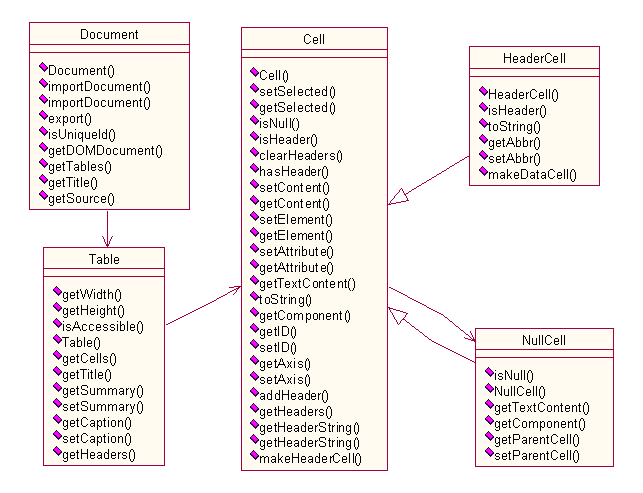
\includegraphics[width=150mm]{figures/document-class-diagram.png}
\caption{Document Class Diagram}
\label{fig:document-class-diagram}
\end{figure}

\begin{figure}
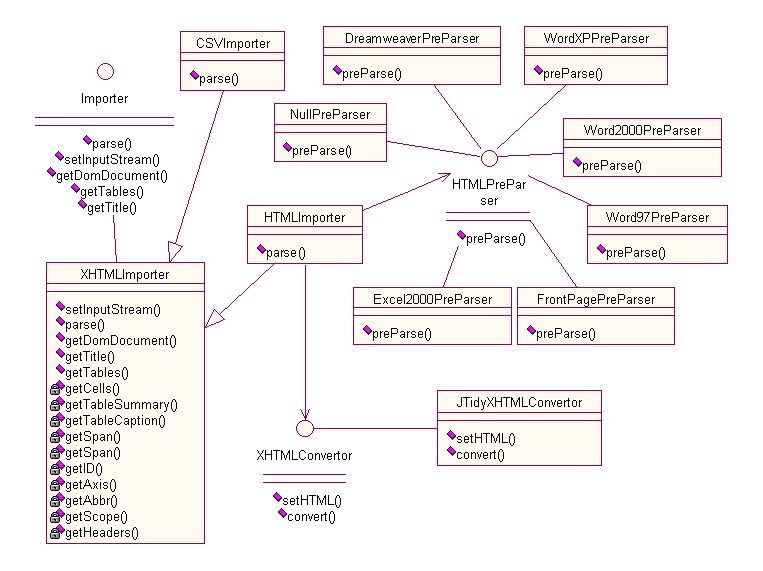
\includegraphics[width=150mm]{figures/import-class-diagram.png}
\caption{Import Class Diagram}
\label{fig:import-class-diagram}
\end{figure}

\begin{figure}
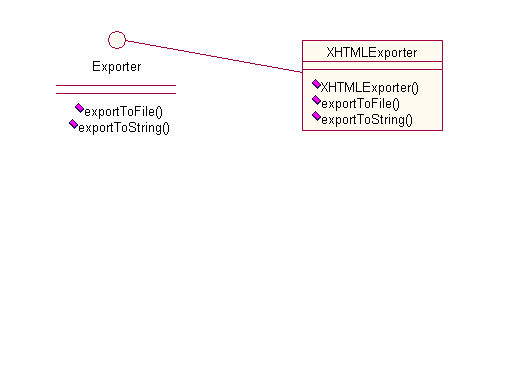
\includegraphics[width=150mm]{figures/export-class-diagram.png}
\caption{Export Class Diagram}
\label{fig:export-class-diagram}
\end{figure}

\begin{figure}
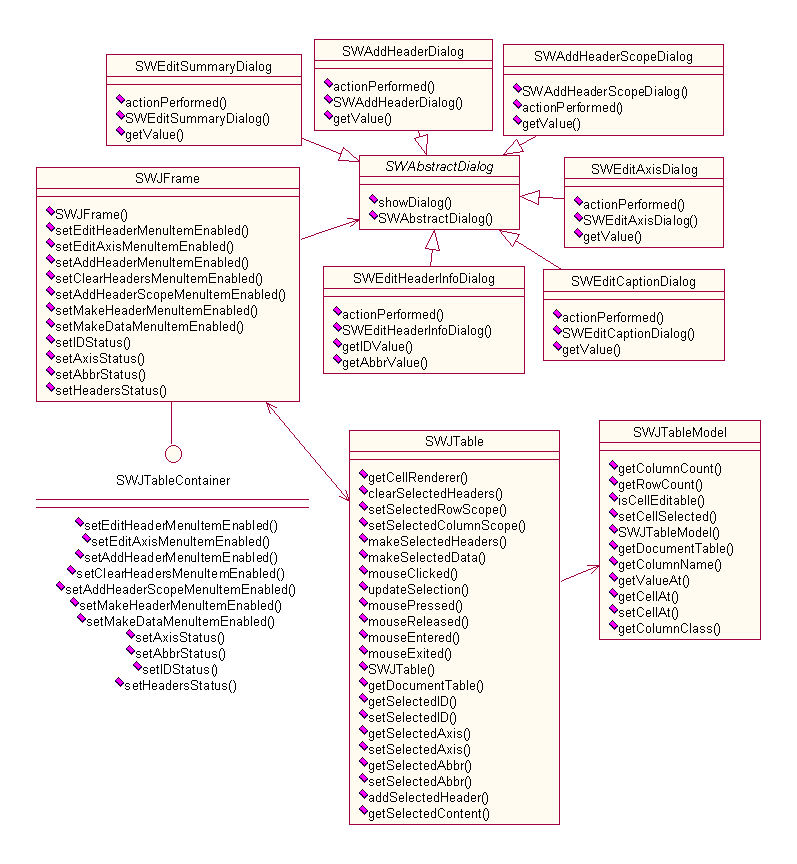
\includegraphics[width=150mm]{figures/gui-class-diagram.png}
\caption{Graphical User Interface Class Diagram}
\label{fig:gui-class-diagram}
\end{figure}



\chapter{Implementation}
% $Id: implementation.tex 269 2003-04-22 14:45:04Z mackers $

\section{Road-map}

The project road-map will roughly adhere to the following sequence:

\begin{enumerate}

\item The project will be begin with the testing and evaluation of the external
tools, components and libraries chosen to complement the table repair tool.
This will reveal at an early stage if the tools are suitable; that is, do they
integrate into the program satisfactorily, and do the results meet what is
required of them. If they do not meet the requirements then other tools must be
investigated or the requirements altered. A short description of each external
component follows:

\begin{itemize}

\item Probably the most important external library is JTidy, used for converting
HTML documents to XHTML. JTidy must be tested for robustness in converting generic
HTML and whether it is compatible with the ``Pre-Parser'' concept. JTidy must not
remove existing accessibility information from the document.

\item The CSV to XHTML convertor should be tested to determine if it is suitable
and robust enough to use in the project.

\item Xerces is a java XML parser that is considered to be more faster and more
sophisticated than the built-in java XML parser. This library should be tested
for compatibility with the standard java DOM classes.

\item Although Swing is built in to java, it does not necessarily have to be
used. It should be tested to see if it is suitable for this project, particularly
the table display component and its accessibility features.

\item CVS\footnote{Concurrent Versions System -- http://www.cvshome.org/} should 
be used to maintain version information and allow for easy backup.

\end{itemize}

In addition, Java's localisation and javadoc features will be examined to see
if they can be used with this particular project.

\item To begin the actual coding stage, a ``bare-bones'' version of a single
document importer will be implemented.  The XHTMLImporter is the most suitable
choice, as it takes the least effort to import (i.e. using the XML parser). At
this stage, the importer will be able to read the document and extract the most
basic information such as normal (non-spanned) cells, and the table summary and
caption. Some sample XHTML documents are created at this stage.

\item Now that an internal representation of a table is available, a basic
graphical user interface should be developed to display the basic table, in
order to ensure that the internal representation is consistent with the
actual table in the document. It is important to have a graphical representation
at this stage as it would be difficult or impossible to view the overall table using
traditional debugging methods.

\item Once the basic table model is implemented and working, further features
can be added to the table backend:

\begin{itemize}

\item Cells in the table should be checked for cell and row spanning and handled
according to W3C HTML recommendations\cite{w3c:xhtml}. 

\item If the document is missing headers, use the header finder algorithm as described
in the requirements.

\item The importer must take into account existing accessibility information in 
the table. Scopes, headers associations, axes and abbreviations must be preserved
and stored in the table or cell objects.

\item If the table accessibility information for table header associations is missing
or incomplete, find this using the heuristic algorithms described in the 
requirements.

\end{itemize}

\item The user interface should be updated to use the new features from the previous
step:

\begin{itemize}

\item The user interface will take spanned cells into account when rendering
the table, either by spanning them as in browsers, or rendering spanned cells
distinctly.

\item The table status bar is implemented to show the attributes of the currently
selected cell(s). This also requires the cell selection mechanism to be implemented.

\end{itemize}

\item After these basic requirements have been implemented, the rest of the graphical
user interface should be added so that subsequent features can be easily tested:

\begin{itemize}

% -- moved to problems -- \item In the user interface window large tables should scroll.

\item Table switching provided via the table menu.

\item The application title bar should consist of application title, document title and table title.

\item Table menus and menu-items should be enabled or disabled by context of open/closed document
and selected cells as described in requirements.

\item The interface and actual functionality of the dialogs.

% -- moved to problems -- \item File filters for the ``Import'' dialog, e.g. ``*.html''.

% -- moved to problems -- \item The mouse cursor should change to the ``Hourglass'' during imports, as they may take
%a short while in which the application would appear to be doing nothing.

\end{itemize}

\item The HTML importer is now ready to be implemented. This should be a
trivial matter, as JTidy has already been tested, and the XHTML importer has
been implemented. In theory, JTidy will open the HTML and give back XHTML,
which can be used by the XHTML importer. Pre-parser support should also be
implemented at this stage. 

\item The CSV importer will also be implemented (using the CSV to XHTML convertor).

\item The XHTML exporter will now be implemented. This should be relatively
trivial as the document's tables and cells have been keeping a record of their
DOM structure to reflect each automated or user change. This means that a
current DOM document is available to export. It might be desirable to use
JTidy's ``pretty-printer'' to output aesthetic XHTML (i.e. indented, etc.).
The ``View Source'' feature, which uses the exporter, should be implemented at
this stage.

\item Now that all the main requirements of the tool have been implemented, the
usability can be focused upon. This includes providing meaningful feedback for
errors when importing and exporting documents. The dialog descriptions are also
entered (if not already).

\item Finally, any remaining Swing accessibility features are added. This includes adding
mnemonics to menus and buttons, adding descriptions to menu items and menus and ensuring
all labels are correctly associated with a menu item.

\item Any remaining javadoc documentation should be added now.

\end{enumerate}

\section{Samples}

The sample set consists of a series of files that will be used for testing
the program's import function as to whether it meets the requirements. The
files will also expose any bugs in the software. 

The criteria for the sample set is as follows:

\begin{enumerate}

\item Documents outputted from each of the supported programs identified
in the requirements section.

\item Tables containing all the accessibility features that are 
required to be retained during the import process, e.g. scope, headers, axis
and abbreviation.

\item A table with column groups.

\item A table with rows shorter than others.

\item A table with headers marked up as bold.

\item A table with a `thead' element instead of headers.

\item A table with no headers or header associations.

\item A table with cells spanning rows and columns.

\item A document with multiple tables.

\item A document with (non-accessible) text outside of a table.

\item A document with a nested table.

\item A document using a layout table.

\item A document with no tables.

\item At least one sample should be an XHTML file.

\item A Word document in its native format.

\item A sample CSV file.

\item A sample unsupported file.

\item Several mal-formed HTML files to test JTidy (these are not including
in the sample set).

\end{enumerate}

\section{Problems Encountered}

During the development of the program, several problems were encountered.
These, together with their solutions, are documentated below.

\label{problems}

\subsection{Localisation}

\begin{itemize}

\item The first issue that became evident was the problem with hard coding
English-language text in the user interface. If, at some future stage, the
program needed to be \emph{localised}, i.e. translated into another language,
then all user interface text in the program would have to be located and
translated in the source code, requiring a recompilation. This would be a time
consuming and tedious task. Instead, all English-language user interface
strings were placed into a \emph{String-Bundle} file and loaded via the
String-Bundle interface. Should a localised version be developed, the human
translator need only translate those strings in the file and rename the file
appropriately and java will use that file instead.

\item From this it also became clear that menu and buttons mnemonics (i.e. 
shortcut keys) could not be hard-coded into the application, as they would 
be different for every language. For example, in English, the mnemonic
for the ``File'' menu would be `F', whereas in Spanish, the mnemonic for
the same menu (``Archivo'' when localised) would be `A'. To this end, the
menu, menu item and buttons mnemonics were also placed in the localised
String-Bundle file.

\item Long text fields presented a problem during the localisation process.
When the length of the text is known, it is possible to split the text so that
it appears correctly and does not stretch the size of the dialog or become
truncated. However, it is more difficult to control the layout of the text when
it must be loaded from a String-Bundle file. For short texts a backslash-n was placed
in the string to cause the Swing component to insert a new line. For longer
texts it was discovered that Swing's JLabel can render a string as HTML, thus
causing it to \emph{wrap} correctly inside the dialog or interface. As a
result, long texts are now represented as in-line HTML documents in the
String-Bundle file.

\item Also, because the main dialogs are being implemented from scratch, the
text and keys for the default ``OK'' and ``Cancel'' buttons must be localised,
whereas normally a dialog using the standard JOptionPane constructs would
handle this.

\item The French language bundle is included with the program. If the operating
system's locale is set to French, then Java will automatically select this
locale to use, and the dialogs and user interface strings will appear in
French. Without having to resort to changing the whole operating system's
locale, the French language bundle can be tested by invoking the java command
with the ``user.language'' system property set to `fr' and the ``user.region''
system property set to `FR'.

\end{itemize}

\subsection{Importing Tables}

\begin{itemize}

\item The HTML, XHTML and CSV importers have been implemented in this release
of the program but the RDF importer has not. It would be desirable to allow
for this importer to be implemented at a later stage, perhaps by a third person
without any alteration of the existing code. 

This required the program to \emph{test} whether the class existed or not.
Regular java code would create a new instance of the RDFImporter using the
\code{new} keyword in order to use it.  However, this would give a compilation
error as the class doesn't exist. Instead the \code{newInstance()} method of
Java's \code{Class} class is used to create the instance of RDFImporter. If the
class has been implemented then it can be used. Otherwise, an exception can be
caught and the user informed that RDF is not available.

\item The Pre-Parser stage of the HTML importer requires a knowledge of the
program in which the HTML was originally created. The requirements section of
this document stated that this should be taken from the document's `Generator'
meta tag. In practice, however, extracting the value of this attribute poses a few problems. Firstly, the case of
the element, attribute name or attribute value may be lowercase, uppercase or a
mixture of the two. Secondly, quotes around the attribute value may be single
quotes, double quotes or missing altogether. The various supported programs
generate a combination of all these problems. It was concluded that the best
means to extract the exact generator attribute value was via a \emph{regular
expression}. Regular expressions are a powerful way to match patterns in
strings of text. In this case, the regular expression is used to match
case-insensitively with optional quotes around the attribute values.

\item The ``Make Header'' and ``Make Data'' features need to change the tag
name of the cell in the document's DOM. However, there is no DOM function
to change a tag's name. This necessitated a new function to do this, which 
consisted of the cloning of the old element's child nodes and attributes into
a new element with the new name and swapping them in the DOM tree.

\item A seemingly intermittent problem occurred when importing XHTML files.
Upon attempting to load and parse the XHTML file, a
\emph{NoRouteToHostException} was being thrown. After some investigation, it
was realized that this problem was only occurring on certain machines, that is,
those without a direct external connection to the Internet. What was in fact
happening, was that the XML parser was attempting to download the XHTML
DTD\footnote{The DTD file is used to check the XHTML file for \emph{validity}
and has a uniform worldwide location of
http://www.w3.org/tr/xhtml1/Dtd/xhtml1-strict.dtd} and was unable to because it
was unaware of the proxy settings needed. To overcome this problem, java
needed to be started with the system \code{http.proxyHost} and \code{http.proxyPort}
settings defined correctly.

\end{itemize}

\subsection{Graphical User Interface}

\begin{itemize}

\item Selected table cells are indicated by a different background colour
(light blue). This was implemented by returning a new cell component albeit
with a different background colour. However, this only set the background
colour behind the text and not in the whole cell, which looked a bit
unconventional and unintuitive. The cell component was then set to be the
maximum possible size, meaning that it would stretch inside the table cell
and the background colour would include the entire area.

\item Large tables caused a problem with the table display mechanism. If the
number of rows exceeded the size of the application window, then Swing would
reduce the height of all the rows to make room. This resulted in unreadable
text, which was problematic in conveying the header information to the user.
This problem was solved by placing each table in a \emph{ScrollPane} which
provides a vertical scrollbar which does not force Swing to squash the table
rows and can be used by the user to scroll the table up or down to reveal
the rest of the table.

\item Each cell renders the first text node found in the corresponding cell in
the table in the import document. However, if text in the cell is within
another element, for example a paragraph or bold element then this is not
returned by the appropriate DOM function. A new DOM function was written to
return \emph{all} text found in the context of the cell, including that found
in sub-elements. This ensured that the cell's made sense in all contexts.

\item Some importers take a short while to open and parse the document. This is
especially noticeable with the HTMLImporter, which must call JTidy to convert
the import document. During this time, the application does not appear to do
anything, even to ``hang'' momentarily. Depending on the size of the document,
the user may be unaware of what is happening and may believe something has gone
wrong as the program is not responding. To overcome this ambiguity, the mouse
cursor is temporarily changed to the wait or `hourglass' cursor while the
document is being imported. This provides visual feedback to the user who knows
that something is happening in the background and that he/she must wait.

\item The application was developed on a Linux system using the default
Swing application look-and-feel. For experienced Linux users, this interface
poses no problem as they are used to and feel comfortable with a range of
different look-and-feels. However, Windows users may not be entirely 
comfortable with strange interfaces. To this end, the program now uses the
`system' look-and-feel, which causes Swing to render components differently
depending on the operating system under which it is run.

\item Testing the software in Windows revealed that the JTable was rendered
slightly different than during development, in that blank JTable headers 
were displayed. This was fixed.

\end{itemize}

\subsection{Packaging}

\begin{itemize}

\item The program is to be deployed as a JAR archive file, and testing as this
revealed some problems. The first problem was that the ``.properties'' 
String-Bundle files were not correctly loaded, resulting in blank user interface
strings. This problem was solved by adding a package qualifier to the function
loading these files.

\item Also, the default class to run should be specified in the JAR file, as this
simplifies the execution of the program. This involved creating a \emph{Manifest}
file for the JAR package which stated which was the default class to run.

\end{itemize}


\chapter{Analysis}
% $Id: evaluation.tex 269 2003-04-22 14:45:04Z mackers $

\section{Evaluation}

The testing of the program took part in two stages; validation and
verification. 

\subsection{Validation}

Validation concerns itself with testing the specification against the user
requirements. By taking each of the user requirements in turn and comparing to
the system requirements it can be determine if the product is \emph{valid},
that is, the correct product has been built. 

By careful comparison of the the user requirements in this document (starting
on page \pageref{userreqs}) to the system requirements (starting page
\pageref{sysreqs}), it is evident that, yes, the product is indeed valid, as
all user requirements have been addressed in the specification.

\subsection{Verification}

Verification means testing the product against the specifications, that is, is
the product being built correctly. Each system requirement must be implemented
in the final program, which should, at the very least, function as expected in
the specification. 

As well as correctly handling the sample test cases that are tested with it,
the verification stage should ensure that the program is robust enough to
handle any input within the bounds of the requirements.

Furthermore, fulfilling the requirements means that the program must act within
the requirements for all situations and circumstances. Any problems that occur
in the problem as a result of an unanticipated user action mean that the
program does not meet its requirements. This requires that the program be
thoroughly tested to identify and eliminate all software flaws or ``bugs''.

\subsection{Program Testing}

\begin{quotation}

Program testing can be a very effective way to show the presence of bugs,
but it is hopelessly inadequate for showing their absence.\cite{dijkstra}

\end{quotation}

It is impractical and superfluous to list all the tests that were performed
on the program here. Instead, the \emph{testing process} that the software
was subjected to is described below.

Testing should always involve a hypothesis; to see if the program behaves
correctly under certain circumstances, load or situations. In each test, it
should be known what is being tested and what is expected to happen. Each
test was designed to test a single aspect or hypothesis and was placed into
one of the following categories:

\begin{itemize}

\item Correctness -- the rightness of the algorithmic functions.

\item Reliability -- how often it fails.

\item Robustness -- how it tolerates changing conditions.

\item Performance -- how fast it is.

\item Usability -- how good the user interaction is.

\item Utility -- how good is it at doing what it is supposed to.

\end{itemize}

Looking for software bugs can be a tedious process, so it helped to narrow the
search to some likely places that they are likely to occur in. Things that
``couldn't possibly happen'' usually do at some stage, the so-called
``exceptional cases''. ``Boundary cases'' were also considered. For instance,
something which works for the values of 2,3,4 and 5 should be tested with 0, -1
and 1,000,000. Also, a large part of the testing concentrated on user input;
users often do unexpected things.

Another stage of the testing was looking at the javadoc comments for each
function to try and find any weaknesses. For example, if the documentation said
``don't do x'' then `x' was done. Large-scale abuse of the functions were
attempted in order to find flaws. Empty strings, negative numbers and
null-references are all examples of something which may break the code.

Each flaw that was discovered was fixed in isolation. By changing one thing
at a time, the consequences can be predicted and can be compared before and 
after. \emph{Regression testing} after each test ensured that fixed a particular
flaw did not introduce any new problems.

\subsection{Domain Testing}

Of course, the main requirement of the program is to output accessible HTML
tables.  For testing the program's output, each sample document was put through
the program, using typical or suitable values where user input was required. The
output was then evaluated using three metrics; manual inspection, automatic
inspection and field testing. 

\subsubsection{Manual Inspection}

The manual testing stage involved inspecting the HTML source of each processed
document for the required accessibility information and testing against the
project's WCAG and Section 508 requirements. In this stage, only the table's
accessibility information was inspected. The manual testing results are shown
in table \ref{table:manual-inspection}. There were only two test failures, and
these can be explained by bug 0012 (see section \ref{knownissues}).

\begin{table}
\small
\begin{tabular}{lccccc}
\strong{Sample} & \strong{Caption} & \strong{Summary} & \strong{Headers} & \strong{Abbr.} & \strong{Axis} \\
boldheaders-sample1 & Pass & Pass & Pass & N/A & N/A \\
colgroup-sample1  & Pass & Pass & Pass & Pass & N/A \\
colgroup-sample2  & Pass & Pass & Pass & Pass & N/A \\
demonstration-sample1-word2000  & Pass & Pass & Pass & Pass & N/A \\
demonstration-sample1-word97  & Pass & Pass & Pass & Pass & N/A \\
general-sample1-word97  & Pass & Pass & Fail & Pass & N/A \\
headers-sample1  & Pass & Pass & Pass & Pass & Pass \\
layout-sample1  & \multicolumn{5}{c}{N/A} \\
multiple-sample1  & Pass & Pass & Pass & Pass & Pass \\
nested-sample1  & \multicolumn{5}{c}{N/A} \\
notable-sample1  &  \multicolumn{5}{c}{N/A} \\ 
scope-sample1  & Pass & Pass & Pass & Pass & N/A \\
spanning-sample1-excel2000  & Pass & Pass & Fail & Pass & N/A \\
spanning-sample1-word2000-a  & Pass & Pass & Pass & Pass & Pass \\
spanning-sample1-word97  & Pass & Pass & Pass & Pass & Pass \\
spanning-sample1-wordxp  & Pass & Pass & Pass & Pass & Pass \\
spanning-sample1  & Pass & Pass & Pass & Pass & Pass \\
thead-sample1  & Pass & Pass & Pass & Pass & N/A \\
\end{tabular}
\caption{Results of Manual Inspection Testing}
\label{table:manual-inspection}
\normalsize
\end{table}

\subsubsection{Automatic Inspection}

The automatic inspection stage involves running the outputted documents through
two validation programs; the W3C validator and Bobby (see section
\ref{relatedwork}). The W3C validator was allowed to detect the
document type (i.e. XHTML) but the character encoding was set to ``UTF-8''.
Bobby's WCAG 1.0 compliance level and U.S. Section 508 compliancy is shown. The
validation and accessibility errors are marked in table \ref{table:automatic-inspection}
and explained below. It should be noted that the errors in the documents do not
present any significant problems to the operation of screen reader software.

\begin{description}
\item \footnotemark[1] This document did not validate because there is one or more duplicate 
header ID as a result of bug 0002 (see section \ref{knownissues}) 
\item \footnotemark[2] This document did not validate because the headers attribute is empty. 
This is an indirect symptom of bug 0012.
\item \footnotemark[3] This document does not conform to WCAG 1.0 because there is 
inaccessible content outside of the table(s) (not introduced by the program).
\item \footnotemark[4] This document does not conform to WCAG 1.0 because the table contains
an absolute width (not introduced by the program).
\end{description}

\begin{table}
\small
\begin{tabular}{lp{25mm}p{25mm}p{25mm}}
\strong{Sample} & \strong{W3C Validator} & \strong{Bobby WCAG} & \strong{Bobby S.508} \\
boldheaders-sample1 & Valid & AA\footnotemark[3] & Approved\\ 
colgroup-sample1 & Valid & AA\footnotemark[3] & Approved \\
colgroup-sample2 & Valid & AA\footnotemark[3] & Approved \\
demonstration-sample1-word2000 & Not Valid\footnotemark[1] & AA\footnotemark[3]  & Approved \\
demonstration-sample1-word97 & Not Valid\footnotemark[1] & A\footnotemark[4] & Approved \\
general-sample1-word97 & Not Valid\footnotemark[2] & A\footnotemark[4] & Approved \\
headers-sample1 & Valid & AAA & Approved \\
layout-sample1  & \multicolumn{3}{l}{N/A} \\
multiple-sample1 & Not Valid\footnotemark[1]\ \footnotemark[2] & AAA & Approved \\
nested-sample1  & \multicolumn{3}{l}{N/A} \\
notable-sample1  & \multicolumn{3}{l}{N/A} \\
scope-sample1 & Valid & AA\footnotemark[3] & Approved  \\
spanning-sample1-excel2000 & Not Valid\footnotemark[1] & A\footnotemark[4] & Approved \\
spanning-sample1-word2000-a & Valid & AA\footnotemark[4] & Approved \\
spanning-sample1-word97  & Not Valid\footnotemark[1] & A\footnotemark[4] & Approved \\
spanning-sample1-wordxp & Valid & A\footnotemark[3] & Approved \\
spanning-sample1 & Valid & AAA & Approved \\ 
thead-sample1 & Valid & AA\footnotemark[3] & Approved \\
\end{tabular}
\caption{Results of Automatic Inspection Testing}
\label{table:automatic-inspection}
\normalsize
\end{table}

\subsubsection{Field Testing}

The document outputs were also tested with actual screen readers in order to
get an appreciation of how the tables will be experiences ``in the field''.
Three screen readers were used for this stage of testing;
JAWS\footnote{http://www.freedomscientific.com/fs\_products/software\_jaws.asp},
IBM Home Page Reader\footnote{http://www-3.ibm.com/able/hpr.html} and Simply
Web 2000 \footnote{http://www.econointl.com/sw/}. Both `before' and `after'
versions of the documents were tested, to see if the process improved their
accessibility from the screen reader's point of view. 

The results were disappointing, in that there was no significant difference 
in the speech output of the document after it had been `accessibilised'. However,
this is mainly due to the limitations of the screen reader programs, which do
not take full advantage of the new accessibility information embedded in the 
document. Some of the programs used some of the accessibility features, and
these results are shown in table \ref{table:field-testing}.

However, some consolation can be taken from the fact that the program did not
interfere with the screen readers' reading of the document. Hopefully, as 
the screen readers improve, they will be able to take advantage of the
accessibility information that is `hidden' in the documents outputted by
this and other programs.

\begin{table}
\small
\begin{tabular}{lp{20mm}p{20mm}p{20mm}p{20mm}p{20mm}}
& Summary & Caption & Headers & Abbrev. & Axis \\
JAWS & Yes & Yes & No & No & No \\
IBM HPR & No & Yes & No & No & No \\
SW2000 & No & Yes & No & No & No \\
\end{tabular}
\caption{Screen Reader Utilisation of Table Accessibility Features}
\label{table:field-testing}
\normalsize
\end{table}

\subsubsection{ATAG Conformance}

The program was also tested to see if it meets the authoring tool
guidelines\cite{w3c:atag}. Each guideline is given below, together with
a verdict and explanation of how the program conforms or not.

\subsubsection{Guideline 1. Support accessible authoring practices}

Yes. The tool automatically generates accessible markup together with 
guiding the user in producing accessible content.

\subsubsection{Guideline 2. Generate standard markup}

Yes. The tool generates valid XHTML 1.0 Strict.

\subsubsection{Guideline 3. Support the creation of accessible content}

Yes. The program allows users to provide equivalent alternative
information for tables.

\subsubsection{Guideline 4. Provide ways of checking and correcting inaccessible content}

Yes. The program checks for inaccessible content when at document export time. By its
very nature the program provides ways to correct this.

\subsubsection{Guideline 5. Integrate accessibility solutions into the overall ``look and feel''}

Yes.

\subsubsection{Guideline 6. Promote accessibility in help and documentation}

Yes. Each dialog gives an explanation of the accessibility features.

\subsubsection{Guideline 7. Ensure that the authoring tool is accessible to authors with disabilities}

With the exception of bug 0001 (see below), the tool is fully accessible
using Swing's accessibility standards.

\section{Known Issues}

\label{knownissues}

Some of the most salient problems discovered during the implementation and
testing process are discussed in the ``Problems Encountered'' section of the
previous chapter (page \pageref{problems}). However, not all bugs or issues
discovered were considered critical enough to fix in this release.  These have
been identified below, with consideration to re-addressing them at some stage in
the future (see ``Future Work'', page \pageref{futurework}). 

Each bug is identified with a \emph{bug id}, which is also used to mark the bug
in the program source code. The bug list is sorted by severity of bug, with the
highest priority first. None of these bugs are critical, but they do imply the
program does not meet the system requirements: 

\begin{enumerate}

\item Bug 0001: Cursor keys do not function in the table viewer, resulting in
the need for a mouse for program operation. This means the program is not
in fact ATAG\cite{w3c:atag} compliant.

\item Bug 0018: Layout tables are not identified when imported.

\item Bug 0014: Regular expression for identifying HTML files does not work
as expected.

\item Bug 0002: The user can enter a duplicate ID in the ``Edit Header Info'' dialog.

\item Bug 0012: The ``Make Header'' dialog does not assign the new header a header
ID.

\item Bug 0007: It is possible to import a new document without exporting the current
one. This may result in a loss of data.

\item Bug 0008: It is possible to close the window without exporting the currently
open document. This may result in a loss of data.

\item Bug 0009: A maximum of 10 headers per cell is allowed. Attempting to add another
header should give an error message to inform the user.

\item Bug 0010: Setting header scope to ``row'' on a cell that spans rows does not
set the headers on cells to the right of the spanned cells.

\item Bug 0011: As bug 0010, but with column spanning.

\item Bug 0019: Table menu's list of table captions could exceed the required
12 letters (as in requirements).

\item Bug 0026: Exporting the document does not update the application's title bar
with the new filename.

\end{enumerate}



\chapter{Conclusion}
% $Id: conclusion.tex 269 2003-04-22 14:45:04Z mackers $

\section{What Was Achieved}

A lot of new technologies and skills were learnt during the course of the
project. 

As demonstrated in chapter 2, an extensive understanding of the core
technologies involved was undertaken. This included reading W3C's extensive and
detailed specifications and recommendations for HTML and XHTML and
accessibility guidelines for web content and authoring tools.

There were other, secondary technologies that were learnt as part of the
project implementation. These included using Swing to develop the 
graphical user interface and Xerces has an XML and DOM parser. Javadoc
was also employed to create the project API.

Auxiliary achievements include learning and using CSV as a version control
system for the program source code and learning to use \LaTeX\ to write and
typeset this report.

It was also very interesting and beneficial to go through the whole software
engineering process, from researching a topic, defining requirements and
specifications right through to writing the actual software and evaluating it.
There was an incredible sense of satisfaction and achievement when the project
was successfully completed. 

\section{Future Work}

\label{futurework}

The project as a whole can be said to have reached a level
of stability and completeness; a true ``version 1.0''. However,
this does not preclude the possibility of improvements and
other features being added.

Naturally, the first improvement would be to fix the bugs listed
in the ``Known Issues'' section on page \pageref{knownissues}. All
of these should be fairly trivial to fix.

Other improvements that could be made are listed below. They
were not listed in the known issues list because they were not
part of the original requirements, and did not need to be 
implemented.

\begin{itemize}

\item ``Rowgroup'' and ``colgroup'' scopes could be supported when
importing documents. Although the supported output formats do
not use these attributes, supporting them would mean that the
program supports all table accessibility features. (bug 0016)

\item The user should be informed if the program could not
identify or guess any header information. This would ensure
that the user does not attempt to export the document without
this fundamental information. (bug 0020)

\item In the absence of a table summary, either in the original
document or supplied by the user, the program could generate
the summary based on the number of rows and columns and other
structural information in the table. (bug 0021)

\item The table cell renderer is too slow. This is probably
because each time the table is refreshed a new component
is created for the cell and return to the table renderer.
Instead, the same cell component should be reused. (bug 0025)

\item If a generator tag is present in the imported document,
it is currently replaced with a SightWeaver generator tag.
However, if one is not present, then it cannot be replaced. A
new generator tag should be added. (bug 0023)

\end{itemize}

Here are some other features that the program would benefit from:

\begin{itemize}

\item The RDF importer is currently supported, but not implemented. If one was
to implement this, a ``RDFImporter'' class would be created to implement the
``Importer'' interface, in a similar manner to the ``CSVImporter''. The
compiled class can then just be dropped into the sightweaver package and the
Document class will use this for RDF files.

\item Other importers that could be implemented include a native binary Word
format importer (difficult!), a DOCBOOK importer, etc. 

\item It would also be nice if a URL could be provided to import documents, and
if the exporter could publish directly to the web via FTP or WEBDAV, allowing
the user to use the program as a final step before publishing to the website.

\item Cell spanning is currently ugly and unintuitive. Word and web user are 
accustomed to seeing spanned cells appearing in the same cell, as opposed
to having a placeholder cell instead. In this case, it might be possible
to turn off the cell borders for the spanned cells to give the impression
that the spanned cells are a single cell with text that is top- and left-aligned.
Anything more sophisticated than that would require a more drastic approach
involving moving away from the current JTable approach to manually place the
cells. Using this approach, a single cell could be place anywhere in the
table, allowing the impression that the cell was spanned and has centre- and
middle-aligned text.

\item A feature that would be of great help to content developers with an
accessibility conscience would be a ``screen-reader simulation'' mode. This
would involved a dialog that would either display or speak a version of the
table or document as it would appear to a user using a screen-reader. This
would give confidence to the content developer that his or her tables
actually make sense when viewed in this manner.

\item Large organisations may use an existing content development package or
system that is unsuitable for create accessible content. This program would be
attractive in that situation, as it could convert the existing format to an
accessible one. However, most organisations have a large amount of documents
that would have to be converted; a tedious task if they are all similar but
needed to be converted manually. Ideally, this tool would `learn' from a single
document and be able to apply that to the rest in the document set. This solution
would require a fair amount of clever AI techniques.

\end{itemize}

It is also quite practical for the program to be included as part of another,
larger program. All the functionality of the document import and export
algorithms has been completely separated from the graphical user interface.
Also, the main functionality of the user interface has been modularised into
the SWTable classes, meaning that the actual window itself is merely a holder
for the menus (which simply calls functions of the table) and the status bar
(which is manipulated by the table). By implementing the ``SWJTableContainer''
interface, any other window, frame or other container can be fully compatible
with the bulk of the program. It should also be possible to implement the
program as a web service, however some user feedback is always needed so the 
process can never be fully automated.

As the program is fully internationalisable, it's relatively easy to localise
into different languages. Translators need only make a copy of the
``sw.properties'' file and translate each string therein (with a
couple of marked exceptions). The new file is then saved with a new filename
indicating the language and country code. For example, Austrian German
would be saved in a file called ``sw\_de\_AT.properties''.

It is intended to release the program source code under the GPL\cite{gpl} 
license to encourage and allow people to implement some or all of these
improvements as they see fit.

\section{Conclusions}

Overall, this project can be said to have been successful. The motivation
behind the accessibility movement was presented both from a social and legal
perspective. The report then went on to explain the accessibility standards and
legislation that exists today, as well as the problems with websites as they
stand today. Existing technologies and other related work in the fields of
assistive technology and accessibility tools was then explored.

The report then proposed a solution to one aspect of accessibility; tables. The
solution was in the form of a tool to assist authors in creating fully
accessible tables. The requirements and specification of the tool were
detailed, as well as the architecture and design process. There then followed a
discussion of the problems that occurred during development and the outstanding
issues that remain. The tool was then evaluated against accessibility and legal
standards.

In this chapter, some possible future work in this area was discussed, as well
as what was achieved in the project as a whole.

The reader may additionally wish to peruse this report's appendices, which contain
the day-by-day project diary, the tool's user manual and details on the contents
of the accompanying CD-ROM.


\pagebreak
\addcontentsline{toc}{chapter}{Bibliography}
\bibliography{report}
\bibliographystyle{plain}
\pagebreak

\appendix
% $Id: appendix-b.tex 269 2003-04-22 14:45:04Z mackers $

\setlength{\parindent}{0em}

\chapter{Project Diary}

\subsubsection{Week Starting November 4th}

Background reading of W3C guidelines and reports and other web
tutorials. Wrote draft of ``introduction'' and ``background'' chapters.

\subsubsection{Week Starting November 11th}

Started to create sample set to get broad idea of technologies
involved.

Investigated related work.

\subsubsection{Week Starting December 20th}

Created first ``requirements and specifications'' draft.

\subsubsection{Week Starting January 6th}

Designed project architecture and class structure

\subsubsection{Week Starting January 13th}

Implemented skeletal classes.

\subsubsection{January 21st}

Read the Swing tutorial, played with sample applications and created
first SWJFrame window.

\subsubsection{January 23rd}

Investigated internationalisation features. Created sw.properties file.
Replaced menu names with internationalised versions.

\subsubsection{January 24th}

Played with java Xerces. Added XML/DOM parsing function to XHTMLImporter.
Added temporary ``Debug'' menu to program.

\subsubsection{February 7th}

Preliminary DOM parsing. Code to map table rows and cells to internal
data structures. Summary and caption parsing.

\subsubsection{February 10th}

Worked on table display classes. Implemented \code{getComponent} method
in cells and header cells.

\subsubsection{February 16th}

Implemented \code{NullCell} to add row and column spanning support. Algorithms
for filling cells correctly around spanned cells and short rows. Aligned
with W3C specifications.

\subsubsection{February 17th}

Added cell selection support using a mouse listener on the table. Updated
cell class to change background colour for selected cells.

\subsubsection{February 18th}

Placed tables in scroll pane to allow user to scroll big tables. Added status
bar with placeholder text. Added window title bar text.

\subsubsection{February 20th}

Implemented id/abbr/axis and basic headers importing and hooked this in to
the status bar display code. Table switching now available from table menu.

\subsubsection{March 12th}

Implemented HTML importing using JTidy, a CSV importer and a XHTML exporter
using JTidy's pretty print function.

\subsubsection{March 13th}

Improved header import algorithm to support scopes and theads. Also imported
the header finder algorithm for unclaimed cells. 

Implemented `AI' header finder algorithm using heuristics for detecting
headers marked up as bold, etc.

Spanned cells are now displayed prettily in the user interface and the ``no-mans-land''
is painted white.

Improved exporter to export existing cell attributes and correct tag names
for guessed headers.

\subsubsection{March 14th}

Work on menus; added separators and context enabling based on selected cells, 
as per requirements.

Misc. testing and bug fixing and usability improvements with dialog boxes for
import errors such as nested/missing table testing. Added filters to import
dialog box. Added view source functionality.

Added pre-parsers via ``generator'' regular expression.

\subsubsection{March 15th}

JAR file testing revealed some bugs. Testing on Windows revealed more bugs.

\subsubsection{March 18th}

Dialog day - implemented user interface and functionality of all dialogs, which 
was simply a matter of calling the appropriate methods on the existing document,
table and cell classes.

\subsubsection{March 30th}

Added descriptions to dialogs.

\subsubsection{April 3rd}

Added mnemonics to menus and menu items.

\subsubsection{April 4th}

Added remaining Swing accessibility requirements, such as giving components
accessible names and descriptions where necessary and linking labels to their
related components.

\subsubsection{April 6th}

Added any remaining javadoc comments.

\chapter{User Manual}
% $Id: appendix-a.tex 274 2003-05-07 16:22:37Z mackers $

SightWeaver is a tool for repairing HTML tables so that they comply with
existing accessibility standards. The program imports existing HTML documents,
and attempts to determine accessibility information from the markup. The user
is then presented with the corrected tables and may verify and refine the table
structure and accessibilty information before exporting the document.

Features:

\begin{itemize}

\item Can import XHTML, HTML and CSV files formats. Invalid or badly marked up HTML is supported by using JTidy.

\item Microsoft Word and Excel ``Save-As-HTML'' documents are also explicitly supported.

\item All existing accessibility information in the original document is preserved and re-used.

\item Documents can contain up to 10 tables. Non-table content is preserved and also ``cleaned'' using JTidy.

\item Robust table parser - cell spanning, short rows, thead, etc.

\item The user is given full control over all accessibility information in the tables; including table summaries, captions and cell headers structure, header associations, axes and abbreviations.

\item Output is well-formed, valid XHTML.

\item (Table) output conforms to WCAG and Section 508 web standards.

\item Program conforms to ATAG.

\end{itemize}

\section*{Running the Program}

SightWeaver is a java application and therefore must have the Java Runtime
Environment (JRE) installed in order to use. The JRE can be downloaded from Sun
Microsystem's website\footnote{http://www.sun.com/} . Version 1.4 or greater is
needed to run this program, and it has been tested and operates correctly under
the Windows, Linux and Solaris operating systems.

To start the program, type ``java -jar sightweaver.jar'' in a command prompt or
terminal window. This will start the graphical user interface, which is the
main interface for importing, manipulating and exporting documents.

\section*{Importing Files}

To import an existing document, click on ``Import'' in the ``File'' menu. This
will bring up a standard dialog box, from which the document can be selected.
Supported file types are HTML, XHTML and CSV. The tables must be data tables (as
opposed to layout tables) and must not be nested. If the document does not
contain any tables, the document will not be opened.

Existing table accessibility information in the table will be maintained, and
the program will attempt to guess other informations such as incorrectly
marked up headers, and header associations.

Other document content will also be preserved but will not appear in the 
table window.

\section*{The Table Display}

The first table in the document will be displayed in the table display window.
Other tables can be selected from the ``Table'' menu.

The table is displayed in its \emph{logical} form, so no formatting or styling
information will be displayed. Also, text will be cropped so as to appear in
the table without resizing the cells.

Table \emph{headers} are displayed in a bold font and cells that are
\emph{spanned} are blank with with a diagonal line. 

Cells may be selected by clicking the cell with the left button of the mouse. 
Multiple continuous cells may be selected by clicking again on the next
cell while depressing the ``CTRL'' button.

The following information about selected cells is displayed in the status bar of
the program window:

\begin{itemize}

\item The unique \strong{ID} of the header cell.

\item The \strong{Abbreviation} of the header cell.

\item The associated \strong{Headers} of the header or data cells.

\item The \strong{Axis} of the header or data cells.

\end{itemize}

\section*{Repairing Tables}

The table summary describes the relationship among cells, including their
headers, spanning information or other relationships that may not be obvious
from analysing the structure of the table but that may be apparent in a visual
rendering of the table. The table summary may be edited using the ``Edit Summary''
menu item of the ``Table'' menu.

The table caption is used to describe the table in two to three sentences and may
be edited using the ``Edit Caption'' menu item of the ``Table'' menu.

If the program has not correctly identified the table headers, then these can be
set using the ``Make Header Cell'' menu item. If the program has incorrectly
set the table headers, then use the ``Make Data Cell'' menu item to change
these to data cells.

Cells should be associated with headers in order to identify the relationship
between header and data cells. This can be achieved by selecting the data cells
associated with a header, clicking ``Add Header'' and selecting the correct
header. If all cells under a header can be said to be associated with it, then
this header has a `column' scope. This can be set with the ``Add Header Scope''
menu item. This dialog can also be used to set row scope, which means all the
cells to the right of a header are associated with it.

The table ID is a unique identifier used by cells to refer to their headings
and the header abbreviation should be used to give a terse abbreviation for
headers with long descriptions. These can be set using ``Edit Header Info''.

The cell axis is used to label cells based on some list of categories. Use the
``Edit Axis'' menu item to set this.

\section*{Exporting Files}

Once the table is satisfactory, it may be exported using the ``Export'' menu item
of the ``File'' menu. This displays a standard `Save As' dialog box, from which
the file can be saved as usual. The document will be saved in XHTML Strict 1.0
format, which should be backwards compatible with most browsers.

At this stage, the document will be checked for accessibility. If an error occurs,
a descriptive dialog will be displayed and the document will not be exported.

At any stage during the table repair process, the document HTML source can be viewed
using the ``View Source'' menu item of the ``File'' menu.



% $Id: appendix-c.tex 271 2003-05-02 16:04:07Z mackers $
\chapter{CD-ROM Contents}

The accompanying CD-ROM contains the following:

\begin{itemize}

\item The program source code is included in the ``src'' directory. This
contains all the classes and interfaces needed to compile the sightweaver
package.

\item The program executable is in the root directory of the CD and includes
the sightweaver package as well as the required JTidy and Xerces packages.

\item This report is included in PDF form in the ``doc'' directory.
%For completeness, the original \LaTeX\ source files are including in the ``doc/src'' directory.

\item The slides from the project demonstration are also included in the
``doc'' directory.

\item The program API as generated by javadoc is included in the ``doc/api''
directory. %The API is supplied in HTML and PDF forms.

\item The bugs list is included as a text file in ``doc/BUGS''.

\item Program screen-shots are stored in the ``docs/screenshots'' directory.

\item The sample documents are included in the ``samples'' directory.

\item For convenience, Java 1.4 for various platforms is also included.

\end{itemize}



\end{document}
